\documentclass[11pt]{article}
\usepackage[margin=1in]{geometry}
\usepackage{amsmath,amssymb,booktabs,array,hyperref,graphicx,algorithm,algpseudocode,xcolor}
\newcommand{\R}{\mathbb{R}}
\newcommand{\ustar}{u^{\star}}
\newcommand{\todo}[1]{\textcolor{red}{[#1]}}
% Former working title: CASPER-C: Continuous-Action Preference Elicitation by Reconstruction
\title{\textbf{The Best Question Has No Name:\\Continuous Preference Elicitation in the Latent Space of a State-of-the-Art Recommender}\\[4pt]
\large Paper C (method) --- working draft, long/thesis format\thanks{Earlier working title: ``CASPER-C: Continuous-Action Preference Elicitation by Reconstruction.''}}
\author{}
\date{June 2026}
\begin{document}
\maketitle

\begin{abstract}
\noindent A conversational recommender that asks cold-start preference questions has, in all prior work, chosen each
question from a \emph{discrete} menu: an item, an attribute, or a natural-language aspect. We ask whether the
\emph{action space itself} is a limitation. We replace the discrete question-selector with a \emph{continuous actor}
that emits each question as a free point $q\in\R^{d}$ in the recommender's own item$+$concept embedding space, answered
on a \emph{graded geometric} scale (a continuous response proportional to the projection of the user's latent taste onto
$q$), and trained end-to-end by differentiable unrolling of the question$\to$answer$\to$belief$\to$recommend loop over a
\emph{frozen} recommender. On the exact canonical ruler of our Paper~B testbed, the headline policy reaches
$\mathrm{NDCG@10}$ $0.378$ full / $0.178$ tail. The \emph{fair}, answer-model-matched comparison is against the
strongest \emph{graded} discrete selector (static entropy over the unified pool with graded answers,
\texttt{uent+GRAW}, $0.367/0.158$): the continuous policy wins by $+0.011$ full / $+0.020$ tail; against the discrete
learned SOTA on its native \emph{binary} answers (CASPER-R, $0.360/0.152$) the margin is $+0.018/+0.026$, a comparison
that crosses answer models and is labelled as such. The result is robust to training-seed variation: three independent
retrains give $0.3767\pm0.0012$ / $0.1772\pm0.0021$. We isolate the \emph{per-user adaptive} contribution with a
static-8 control---the strongest fixed continuous questionnaire (eight free directions asked of everyone, built by greedy
selection over the policy's own query distribution, $0.355/0.146$): the genuinely adaptive policy beats it by $+0.023$
full / $+0.032$ tail (${\sim}4\sigma$/${\sim}6\sigma$), and the static bank \emph{inverts} under graded answers (worse
graded than binary), localising the graded-continuity prize to adaptivity. The win is \emph{conditional and instructive}. It requires graded
answers, and the graded channel is not enough on its own: a discrete policy trained on binary answers drops zero-shot
under graded answers; a static discrete heuristic gains a little; and---the decisive control---a discrete policy trained
\emph{natively} on graded answers with full answerability still fails ($0.325/0.125$); only the continuous policy
converts graded answers into ranking gains. Two mechanistic results form the centerpiece. First, \emph{snap-loss}: forcing each
emitted query to its nearest nameable concept costs $-0.037$ full / $-0.040$ tail and drops below the discrete SOTA,
and this is \emph{not} a vocabulary artifact---post-hoc projection onto ${\sim}6.9$M item-pair difference directions,
$9{,}000\times$ more directions, buys $+0.02$ realization cosine and zero NDCG ($0.337/0.134$). Second, a
\emph{realization ladder}: holding the training recipe fixed and varying only the realization set, performance is
monotone in action-set richness (unconstrained $0.378/0.178$ $>$ pair differences $0.370/0.166$ $>$ named entities
$0.356/0.152$, the last a tie with discrete CASPER-R), and \emph{training through the realizer}---straight-through
realization inside the training unroll---rescues most of the snap-loss at every rung. The pair rung is a fully
\emph{askable} interview (``which do you prefer, $A$ or $B$?'' with graded strength-of-preference) at
parity-or-slightly-above the best askable baseline (tail delta positive at every training seed; not per-user
significant, paired bootstrap $p{=}0.30$) and only $-0.008/-0.012$ below the free-direction ceiling. We position this
against the closest prior art (Wolpertinger, ConTS, PEBOL, Vendrov et al.\ 2020, Canal et al.\ 2019), all of which snap
a continuous proto-action back to a discrete catalogue, and argue the contribution is the \emph{un-snapped} off-manifold
query made tractable by the geometric answer---plus the recipe that makes it deployable when a realizable question set
is imposed. We discuss at length what made this strategy \emph{learnable}---the differentiable-unroll approximation,
the reconstruction objective, and the answerability assumption baked into the geometric answer model.
Finally, the headline replicates on MovieLens-25M ($162{,}541$ users, $18{,}430$ items) under a depth-matched
ruler---continuous$+$graded beats the strongest discrete graded selector by a tail gap of $+0.037$, numerically
matching MovieLens-1M.
Finally, we stress-test the whole battery on a \emph{rebuilt, state-of-the-art instrument}---a faithfully replicated
RecVAE (validation $\mathrm{NDCG@100}$ $0.4422$ vs.\ published $0.442$) that on the canonical arena \emph{ties EASE}
($0.554$) while retaining the compact differentiable latent the policy needs (elicitation in a SOTA latent-variable
recommender's latent space is itself without published precedent). The claims do not merely survive on the stronger
instrument; they \emph{sharpen}: continuous beats discrete by $+0.046$ full / $+0.062$ tail, the graded/binary gap widens
into a cliff ($0.491$ vs.\ $0.117$), and the snap-loss grows ${\sim}4\times$ to $-0.147/-0.133$---the off-manifold prize
\emph{grows} with instrument strength. Only adaptivity shrinks (significant on the head, a tie on the tail), exactly as
the linear-Gaussian argument predicts for a stronger, more linear recommender.
\end{abstract}

\tableofcontents

%==================================================================
\section{Introduction}\label{sec:intro}

\begin{figure}[t]
\centering
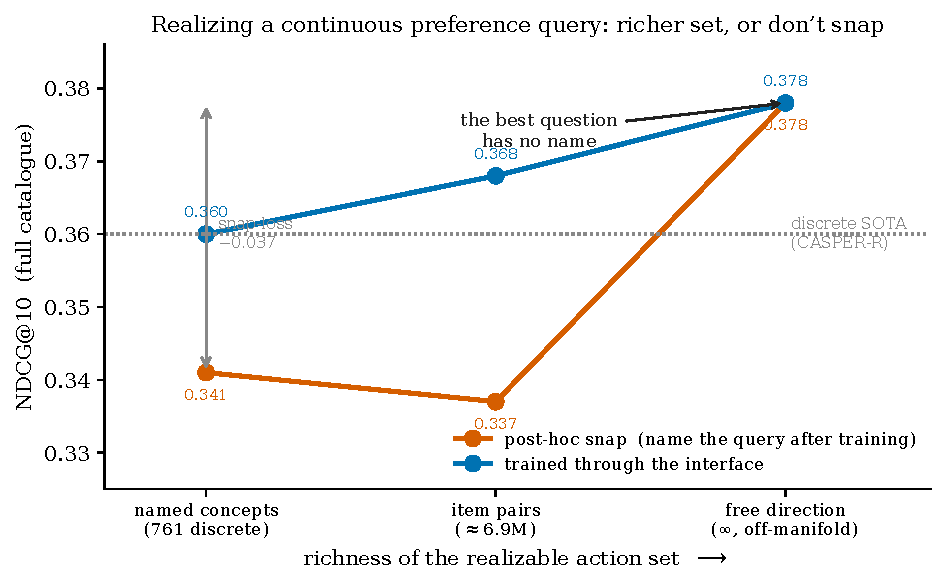
\includegraphics[width=0.86\linewidth]{figs/fig_ladder.pdf}
\caption{\textbf{Graphical abstract: the best question has no name.} As the realizable action set grows richer
(named concepts $\to$ item pairs $\to$ a free continuous direction), elicitation quality (NDCG@10, full catalogue)
rises. \emph{Post-hoc snapping} the continuous query into a named set (orange) forfeits the gain and falls below the
discrete state of the art; \emph{training through the interface} (blue) recovers most of it. Only the un-snapped,
off-manifold direction reaches the top---and the two curves meet there, because a free direction has no interface to
snap through. Numbers: \S\ref{sec:snaploss},~\S\ref{sec:ladder}.}
\label{fig:ladder}
\end{figure}

Cold-start preference elicitation asks a short sequence of questions, folds the answers into a user profile, and then
recommends. Paper~A built a calibrated set-encoder \emph{instrument} (the recommender); Paper~B asked \emph{what to ask}
and established the \emph{answerability} axis---in true cold-start a user can answer broad \emph{concept} questions but
not fine \emph{item} questions---and a learned concept-elicitation policy, \textbf{CASPER-R}, that beats the strongest
divisiveness heuristic on the long tail. Both Paper~A and Paper~B share a structural commitment that this paper
questions: \emph{the question is always chosen from a discrete set}.

\paragraph{The discrete bottleneck.} Whether the menu is items, attributes, or LLM-generated aspects, a discrete
selector can only ask questions that already have a name. Yet the recommender reasons in a continuous embedding space:
a user's taste is a vector $\ustar\in\R^{d}$, and the most informative direction to probe at a given moment need not
coincide with any catalogued concept. If the optimal next question is ``somewhere between \emph{noir} and
\emph{slow-burn revenge}, leaning visual,'' a discrete policy cannot ask it. This paper tests the hypothesis that
\emph{continuous} questions---points in the embedding space, not menu choices---can extract preference information that
the discrete menu cannot, and that this is realisable by a learned policy.

\paragraph{Two coupled continuities.} The proposal has two parts that turn out to be inseparable: a continuous
\emph{action} (the query $q$) and a continuous \emph{answer} (a graded geometric response). A graded answer carries
strictly more information than a binary like/dislike, but the graded channel alone is not the story: a discrete policy
trained on binary answers \emph{drops} zero-shot when fed graded answers; a static discrete heuristic gains a little
(\texttt{uent+GRAW}); and a discrete policy retrained \emph{natively} on graded answers with full answerability still
fails (\S\ref{sec:ablations}). Only the continuous policy converts the graded answer into ranking gains. The
contribution is therefore the \emph{pair}: continuous question $+$ continuous answer.

\paragraph{Contributions.}
\begin{enumerate}
  \item A \emph{continuous-action} elicitation policy that emits questions as free embedding-space points and is trained
  by differentiable unrolling over a frozen recommender, with a geometric graded answer model (\S\ref{sec:method}).
  \item On the \emph{exact} canonical Paper~B ruler (baselines reproduce their published numbers), the policy beats the
  strongest answer-model-matched \emph{graded} discrete baseline (\texttt{uent+GRAW}) by $+0.011$ full / $+0.020$ tail,
  and the discrete learned SOTA on its native binary answers (CASPER-R) by $+0.018$ full / $+0.026$ tail; the result is
  stable across three independent training seeds ($0.3767\pm0.0012$ / $0.1772\pm0.0021$) (\S\ref{sec:main}).
  \item A \textbf{continuous divisiveness field}---the discrete entropy heuristic written in closed form as a smooth,
  differentiable function of a direction and folded into the training reward---which \emph{stacks} on top of continuity:
  continuity alone reaches $0.370/0.165$, the divisiveness reward lifts it to $0.378/0.178$ (\S\ref{sec:main}). It is the
  signal as a \emph{reward}, not as a candidate-scoring feature, that wins.
  \item The \textbf{snap-loss} result: the gain is carried by \emph{off-manifold} queries; snapping to the nearest
  nameable concept destroys it and drops below discrete---so emit-then-snap methods cannot achieve it---and the loss is
  \emph{not} a vocabulary artifact: post-hoc projection onto ${\sim}6.9$M item-pair difference directions loses just as
  much (\S\ref{sec:snaploss}).
  \item The \textbf{realization ladder}: one training recipe, one variable (the realization set). Performance is
  monotone in action-set richness (unconstrained $>$ pair differences $>$ named entities, the last tying discrete
  CASPER-R); \emph{training through the realizer} (straight-through realization inside the unroll) rescues most of the
  snap-loss at every rung; and the pair rung yields a fully \emph{askable} interview at parity-or-slightly-above the
  best askable baseline (\S\ref{sec:ladder}).
  \item The \textbf{static-8 control} that \emph{isolates per-user adaptivity}: against the strongest fixed continuous
  questionnaire under the same objective and graded answer model (eight free directions asked of everyone, built by
  selection over the policy's own query distribution), the adaptive policy wins by $+0.023$ full / $+0.032$ tail---the
  single largest clean effect in the paper---and the static bank inverts under graded answers, localising the
  graded-continuity prize to adaptivity; an effective-rank analysis ($2.25/64$ concepts vs.\ $27.1/64$ items) explains
  why fixed banks saturate while the policy re-aims each turn (\S\ref{sec:static8}).
  \item Ablations isolating \emph{what made it learnable}: the training objective (reconstruction vs.\ ranking vs.\
  divisiveness vs.\ distillation), the answer model (graded vs.\ binary, including a discrete policy trained natively on
  graded answers), and the off-manifold freedom (\S\ref{sec:ablations}).
  \item A characterisation of the realisable ceiling and the privileged oracle headroom, and an extended novelty
  discussion against the nearest prior art (\S\ref{sec:discussion}).
  \item A \textbf{cross-dataset replication} on full MovieLens-25M ($162{,}541$ users, $18{,}430$ items, freshly
  trained instrument and from-scratch actor) under a pre-stated depth-matched ruler ($K{=}50$): the headline gap
  ($+0.024$ full / $+0.037$ tail), the graded/binary inversion, snap-loss, the anti-saturation $q$-curve, and
  saturation-at-effective-rank all replicate, with the tail gap numerically matching ML-1M (\S\ref{sec:ml25m}).
\end{enumerate}

%---- WORKED EXAMPLE BOX: the question that has no name --------------------------
\begin{figure}[t]
\centering
\fbox{\begin{minipage}{0.94\linewidth}
\small
\vspace{2pt}
\textbf{\textsf{The question that has no name}} \hfill {\footnotesize\itshape one real emitted query, V1-era artifacts}\\[3pt]
At one turn the continuous actor emits a direction $q\in\R^{64}$ in the recommender's own space. It is not any catalogue
concept---here is everything we can say about it.\\[4pt]
\begin{tabular}{@{}p{0.30\linewidth}p{0.63\linewidth}@{}}
\toprule
\textbf{What it is} & \textbf{Its shadow on things we \emph{can} name}\\
\midrule
Sparse phrase blend (OMP-3) &
$-0.45\,[\text{Cliff DeYoung}]\;\;+0.41\,[\text{Tim Burton}]$\newline
$-0.35\,[\approx\text{mother-son}\cdot\text{free speech}\cdot\text{nocturnal}]$\\[3pt]
Nearest single \emph{concept} & $[\text{oscar (best sound)}]$, $\cos=0.35$ --- nothing named is close\\[2pt]
Nearest of all $6{,}724$ phrases & $[\text{Teri Garr}]$, $\cos=0.39$\\[2pt]
Best of ${\approx}6.9$M item-\emph{pairs} & \emph{Raiders of the Lost Ark} (1981) vs.\ \emph{The Shop Around the Corner} (1940), $\cos=0.59$\\[2pt]
LLM rendering (axis synthesis) & \emph{``Which do you prefer in a film---a whimsical style like Tim Burton's, or more serious themes?''}\\
\bottomrule
\end{tabular}\\[4pt]
\textbf{The cost of naming it.} Snapping this query to its nearest \emph{concept} before folding costs
$-0.037/-0.040$ NDCG@10 (full/tail); realizing it as the best \emph{item-pair} costs $-0.041/-0.044$ despite a
$9{,}000\times$ larger vocabulary (\S\ref{sec:snaploss},~\S\ref{sec:ladder}). Both land \emph{below} the discrete
state of the art. The query only pays off if it is never named---hence the title.
\vspace{2pt}
\end{minipage}}
\caption{A single continuous query, decomposed. The direction is faithfully \emph{describable} as a signed blend of
familiar phrases (and renderable as one natural question), yet no single concept, phrase, or item-pair \emph{is} it
($\cos\!\le\!0.6$ to the best of each). Naming or snapping it forfeits the gain. Labels are an interpretability layer
over V1-era artifacts; metrics are unchanged by the decomposition.}
\label{fig:worked}
\end{figure}

%==================================================================
\section{Related Work}\label{sec:related}
\paragraph{Conversational and cold-start elicitation.} Classical elicitation is active learning over the
catalogue---pick the item whose rating most reduces uncertainty, by divisiveness, label entropy, or expected
reconstruction-error reduction~\cite{rashid,golbandi11,elahi16}. Modern conversational recommenders (CRS) select a
discrete \emph{item} or \emph{attribute}: EAR, CRM, UNICORN, and the unified item$+$attribute Thompson-sampling policy
ConTS~\cite{lei20ear,sun18crm,deng21unicorn,li21conts}. ConTS is the closest in spirit---it acts in a unified
item$+$attribute embedding space---but its action remains a \emph{discrete argmax over pre-existing arm embeddings};
it never constructs a free query. Our Paper~B (CASPER-R) is also discrete (concepts).

\paragraph{LLM-driven elicitation.} Recent work generates questions with an LLM. PEBOL~\cite{pebol} runs Bayesian
optimisation over LLM-generated \emph{aspects} with binary NLI-scored answers against a frozen LLM; GATE elicits tasks
generatively. These open the \emph{vocabulary} of questions but the action is still a discrete aspect/string and the
answer a single bit; there is no learned continuous policy and no end-to-end training.

\paragraph{Continuous-action RL and the snap.} The natural tool for a continuous action is continuous-action RL.
Wolpertinger~\cite{wolpertinger} emits a continuous proto-action and \emph{$k$-NN snaps} it to a discrete catalogue
before executing; HyAR~\cite{hyar} learns a latent action space but decodes back to a discrete action. The single most
relevant precedent is Vendrov et al.~\cite{vendrov20}: gradient-based Bayesian elicitation relaxes choice-query
\emph{slates} to continuous ``hypothetical items'' in attribute space and optimises a differentiable myopic expected
value of information---but then \emph{projects back to real items} before asking. We differ on three axes: our policy
is an \emph{amortised, learned} non-myopic actor (not a per-step inner optimisation); it acts against a \emph{frozen
neural} recommender rather than a utility model; and we measure the cost of the projection---the snap-loss---as a
first-class quantity rather than treating projection as harmless. \emph{Every} such method snaps; none acts on,
or benefits from, an off-manifold query. Our pair-difference realization (\S\ref{sec:ladder}) generalises the
Wolpertinger snap from nearest-\emph{item} to nearest-\emph{pair-difference}---a $9{,}000\times$ larger realizable
set---and shows that vocabulary size alone does not close the snap-loss; putting the realizer \emph{inside} the
training loop does. The membership-query-synthesis literature acts off-manifold but its classic
failure is that synthesised queries are \emph{human-unanswerable}~\cite{baum92}---exactly the problem our geometric
answer dissolves.

\paragraph{Pairwise-comparison elicitation.} The pair rung of our realization ladder connects to a long line of work
that elicits preferences by comparisons. Polyhedral adaptive conjoint analysis~\cite{toubia04} treats each choice
question as a cut through the polytope of consistent utility vectors; Canal et al.~\cite{canal19} do active embedding
search via noisy paired comparisons, selecting pairs by acquisition rules (no learned policy); Jamieson \&
Nowak~\cite{jamieson11} establish the adaptive-vs-static sample-complexity separation for ranking from pairwise
comparisons (we cite this as the classical motivation for adaptivity with comparison queries, not as new theory);
dueling bandits~\cite{yue09duel} optimise from pairwise feedback for regret. None of these emits a \emph{continuous
query direction} that is then \emph{realised} as the nearest item-pair difference, and none trains the questioner
end-to-end through a frozen recommender; our pair-native policy is, to our knowledge, the first learned continuous
actor whose executed action is a comparison question.

\paragraph{Differentiable experimental design.} DAD and iDAD~\cite{foster21dad} amortise sequential Bayesian design by
backpropagating through unrolled simulated trajectories over continuous designs, but deliberately carry \emph{no}
explicit belief update and target no recommender. DRE~\cite{dre} is differentiable (Gumbel) but elicits a one-shot
static seed set. Our differentiable unroll of an \emph{explicit belief-tracking} loop jointly with a \emph{frozen
recommender}, in embedding-space cold-start, is unmatched.

\paragraph{Embedding inversion (what we do \emph{not} do).} Vec2Text and GEIA~\cite{vec2text,geia} \emph{decode} an
embedding back to text; both are per-encoder, lossy, and do not work reliably on the sentence encoders we use. We make
no such claim: our interpretability is \emph{retrieval}---snap a query to a mined phrase bank (prototype/concept-direction
style~\cite{tcav})---never inversion.

\paragraph{Positioning.} No prior system (i) emits a novel off-manifold query as its executed action, (ii) answers it
geometrically by projection of latent taste, (iii) trains the full query$\to$graded-answer$\to$belief$\to$recommend loop
by differentiable unroll over a frozen recommender, and (iv) reads off strategy by phrase-bank snap---and, decisively,
none claims that \emph{not} snapping beats the best discrete policy. The contribution is this combination; its
load-bearing, individually novel element is the off-manifold query (\S\ref{sec:novelty}).

%==================================================================
\section{Background and Problem Setup}\label{sec:setup}
\paragraph{The frozen recommender (the ``MF layers'').} We inherit Paper~A/B's set-encoder recommender and keep it
\emph{frozen} throughout. Each item $j$ has a factor $Q_j\in\R^{d}$ ($d=64$) and a popularity bias $b_j$; given a user
belief $u\in\R^{d}$, items are scored
\begin{equation}
  s(j) \;=\; b_j + Q_j^{\top}u,
\end{equation}
ranked, and evaluated by $\mathrm{NDCG@10}$ (full and the Cremonesi long tail, which masks the head $33\%$ by
popularity). The belief is produced by a pooled-attention set encoder $\mathrm{Enc}(\cdot)$ over a set of answered
question \emph{tokens}, each a pair $(\text{embedding}\in\R^{d},\,\text{answer}\in\R)$. An item token is
$(Q_j,\text{residual})$; a concept token is $(E_c,\text{like/dislike})$; a \emph{continuous} query token is
$(q,\,a)$---identical in format. The catalogue is finite: $600$ popular askable items, $761$ genome concepts, ${\sim}3.7$k
rankable items, $6040$ users ($4823$ train, $604$ test; we report \texttt{te[300:]}, $304$ users, seed-averaged over
$\{1,2,3,7,11\}$).

\paragraph{The elicitation loop.} Starting from $u_0=\mathbf{0}$, for $t=1,\dots,T$ ($T{=}8$): the policy proposes a
question; the (simulated) user answers; the answer is folded into the belief; after $T$ turns we rank and score.

\paragraph{The geometric answer model and the answerability assumption.} We simulate a user's answer to a query $q$
\emph{geometrically}: the answer is a monotone function of the projection $\ustar^{\top}q$ of the user's true taste
$\ustar$ onto the query, where $\ustar$ is the fold of the user's \emph{known half} of the profile (the held-out half is
the ranking target and is never folded into $\ustar$). Two variants: \emph{binary} $a=\operatorname{sign}(\ustar^{\top}q)$
(one bit), and \emph{graded} $a = \mathrm{NEG} + (\mathrm{POS}-\mathrm{NEG})\cdot\tfrac{1}{2}\!\left(\cos(\ustar,q)+1\right)$
(a continuous ``how much''). This embeds the answerability assumption of Paper~B: any direction $q$ is
\emph{answerable}---the user can always say how much a soft attribute matches their taste---which is exactly what frees
us from the discrete answerable catalogue. Crucially, $\ustar$ is used \emph{only} to generate the answer and the
training gradient; the policy never sees $\ustar$, so it is realisable (\S\ref{sec:method}).

%==================================================================
\section{Method: A Continuous-Action Elicitation Policy}\label{sec:method}
\paragraph{The continuous actor.} The policy is a small MLP $\pi_\theta:(u,t)\mapsto q\in\R^{d}$ that maps the current
belief and turn to a \emph{query direction}. We $\ell_2$-normalise $q$ and scale it to the mean concept norm so it is a
point of plausible magnitude in the embedding space. There is no menu and no snap: the raw point is folded.

\paragraph{Differentiable unroll.} Because (i) the geometric answer $a$ is a smooth function of $q$ and $\ustar$, (ii)
the encoder fold is differentiable, and (iii) the recommender score is differentiable, the \emph{entire} $T$-step
rollout is differentiable. We therefore train $\pi_\theta$ (and optionally the encoder) by backpropagating a reward
through the whole loop---no high-variance policy gradient. The default objective is \emph{reconstruction}: drive the
final belief to the user's taste,
\begin{equation}
  \mathcal{L}_{\text{recon}} \;=\; 1-\cos\!\big(\mathrm{Enc}(\{(q_t,a_t)\}_{t\le T}),\;\ustar\big),
\end{equation}
which is an unbiased, dense, low-variance surrogate. Reconstruction is a \emph{proxy}: it drives the belief to the true
taste, which is necessary but not sufficient for ranking (NDCG@10 weights the head disproportionately). We therefore add
a \emph{differentiable listwise ranking} term. For each user we score the held-out likes against the top-popular items
(the realistic top-10 competition) and apply a soft-rank (ApproxNDCG) surrogate,
\begin{equation}
  \pi_i(q) \;=\; 1+\sum_{j\neq i}\sigma\!\big((s_j-s_i)/\tau\big),\qquad
  \mathcal{L}_{\text{soft-NDCG}} \;=\; -\,\frac{1}{Z}\sum_{i}\frac{\mathrm{rel}_i}{\log_2(1+\pi_i(q))},
\end{equation}
which is differentiable through the scores $s=b+Q^{\top}u_T$ and hence through the whole unroll. The base objective is
$\mathcal{L}_{\text{recon}}+\beta\,\mathcal{L}_{\text{soft-NDCG}}$ (the \emph{continuity-only} model); the headline model
adds the divisiveness reward introduced next. We ablate both terms in \S\ref{sec:ablations}.
A naive pointwise BCE or a \emph{pure} soft-NDCG (replacing reconstruction) both fail---BCE gives too weak a gradient
through the unroll, and pure ranking reward-hacks the surrogate and collapses; the reconstruction anchor is what keeps the
belief sensible while the ranking term shapes the head. Algorithm~\ref{alg:unroll} summarises training.

\paragraph{An exact continuous divisiveness signal (the headline mechanism).} Divisiveness---the entropy of a question's
like-rate, the very signal the discrete entropy heuristic selects on---is a property of a \emph{direction} and is
computable in closed form for any $q$ from the train-user taste distribution:
$p(q)=\frac1N\sum_i\sigma(\ustar_i\!\cdot\hat q/\tau)$ and $D(q)=H_b(p(q))$. This field reproduces the per-concept
divisiveness exactly at the catalogued concept points and---crucially---extends \emph{smoothly and differentiably}
everywhere off-manifold, so it is the discrete entropy heuristic \emph{extrapolated into the continuous action space}.
Adding $+\lambda\sum_t D(q_t)$ to the unroll loss rewards the actor for asking maximally-informative (divisive)
directions, and shapes this population-level optimal-design signal directly into the policy gradient. This term is the
headline model: it lifts the continuity-only actor from $0.370/0.165$ to $\mathbf{0.378/0.178}$ (\S\ref{sec:main}), the
larger of the two stacked continuous contributions. Two design notes matter. First, the win comes from the divisiveness
\emph{reward} on the plain actor, \emph{not} from exposing divisiveness (or popularity, or average rating) as input
features to a candidate-scoring head: a ``continuous CASPER-R'' variant that proposes a region, generates $K$ candidates,
and soft-selects by learned weights over $[\text{div},\text{pop},\text{rating},\text{belief}]$ \emph{underperforms} the
plain actor ($0.351/0.148$), so we report only the reward form. Second, because a divisive direction is chosen precisely
to split the population $\sim$50/50, its value is realised only when the answer carries graded magnitude---the same actor
under \emph{binary} answers regresses to $0.341/0.125$ (below even the continuity-only actor), so the divisiveness gain is
\emph{more} graded-specific than continuity itself.

\begin{algorithm}[t]
\caption{Continuous-actor training by differentiable unroll (one batch)}\label{alg:unroll}
\begin{algorithmic}[1]
\For{each user $x$ in the batch}
  \State $\ustar \gets \mathrm{Enc}(\text{profile tokens})$ \Comment{privileged taste, used for answer + gradient only}
  \State $u_0 \gets \mathbf{0}$, $\text{toks}\gets[\,]$
  \For{$t=1$ to $T$}
    \State $q_t \gets \pi_\theta(u_{t-1}, t/T)$;\quad $\hat q_t \gets q_t/\|q_t\|\cdot c$
    \State $a_t \gets \mathrm{graded}(\cos(\ustar,\hat q_t))$ \Comment{differentiable in $\hat q_t$}
    \State $\text{toks}.\text{append}((\hat q_t,a_t))$;\quad $u_t \gets \mathrm{Enc}(\text{toks})$
  \EndFor
\EndFor
\State $\mathcal{L} \gets \tfrac1B\sum_x \big[1-\cos(u_T^{(x)},\ustar^{(x)})\big]\;+\,\beta\,\mathcal{L}_{\text{soft-NDCG}}\;-\,\lambda\,\tfrac1T\textstyle\sum_t D(\hat q_t^{(x)})$ \Comment{$\lambda{=}0$: continuity only; $\lambda{>}0$: headline}
\State backprop through the unroll; update $\theta$ \Comment{recommender $Q,b$ frozen}
\end{algorithmic}
\end{algorithm}

\paragraph{What makes the strategy learnable (the approximations).} Three approximations are load-bearing and we state
them explicitly. (1) \emph{Geometric answers} make the simulator differentiable and---more importantly---make every
direction answerable, removing the discrete-vocabulary constraint and the need to ever decode a vector to text. (2)
\emph{Differentiable unroll} replaces model-free RL (which, in our experiments, collapses to the heuristic basin) with a
dense analytic gradient; this is why a from-scratch policy converges at all. (3) \emph{Privileged-but-realisable
training}: $\ustar$ enters only the answer and the gradient, never the policy input, so the trained policy runs from the
belief alone---this is the difference between our policy and an answer-peeking oracle.

\paragraph{Realisability.} At test time the simulated user supplies $a_t$ (the same geometric model); the policy maps
$u_{t-1}\mapsto q_t$ with no access to $\ustar$. Nothing privileged is used at inference.

%==================================================================
\section{Experiments}\label{sec:exp}
\paragraph{Protocol and harmonisation.} All numbers are on the \emph{exact} canonical Paper~B harness, encoder, split
protocol, and metric; we evaluate the continuous actor as an additional mode (\texttt{contactor}) inside that harness so
the baselines reproduce their \emph{published} values (we verified CASPER-R $=0.360/0.152$, entropy $=0.361/0.140$;
a corrupted divisiveness cache had earlier depressed all heuristic/scorer baselines and is corrected here). Seed-average
over $\{1,2,3,7,11\}$, $\mathrm{NDCG@10}$ full~/~Cremonesi tail at $q{=}8$, on the last $304$ test users
(\texttt{te[300:]}; the first $300$ test users are reserved as a validation set for checkpoint selection where a
validation set is used). Table~\ref{tab:hyper} lists the hyperparameters of the headline recipe and of the
realization-ladder runs; all trained policies are persisted as locked, hash-recorded checkpoints alongside the exact
frozen recommender they were trained against.

\paragraph{Seeds and significance methodology.} Two kinds of seed appear in this paper and we keep them distinct.
An \emph{evaluation seed} (the five seeds $\{1,2,3,7,11\}$) randomises the per-user split of the test profile into the
known half (which generates answers) and the held-out half (the ranking target); every reported mean is averaged over
the five evaluation seeds and, unless stated otherwise, the $\pm$ is the standard deviation \emph{across evaluation
seeds}. A \emph{training seed} randomises network initialisation and training-batch sampling (the train/test user split
itself is pinned and never varies with the training seed). The headline policy was retrained under $3$ training seeds
and evaluated under the full $5$ evaluation seeds each ($3\times5$ protocol); training-seed means are labelled as such.
Because every evaluation seed scores the \emph{same} $304$ users, seed-level standard deviations understate per-user
noise; for the deployability comparison of \S\ref{sec:ladder} we therefore additionally run a \emph{paired per-user
bootstrap}: per-user NDCG@10 averaged over the five evaluation seeds for method and baseline on identical users and
splits, then $10{,}000$ bootstrap resamples over the $304$ users, reporting the delta, its $95\%$ CI, and a two-sided
$p$. Where a claim does not survive this test we say so explicitly.

\begin{table}[t]\centering
\begin{tabular}{lll}
\toprule
Hyperparameter & Value & Notes \\
\midrule
Embedding dimension $d$ & $64$ & frozen V1 set-encoder / SVD factors \\
Questions per episode $T$ & $8$ & \\
Divisiveness reward weight $\lambda$ (\texttt{DIVW}) & $1.0$ & headline (D1); $\lambda{=}0$ = continuity-only \\
Divisiveness temperature $\tau_D$ (\texttt{DTAU}) & $2.0$ & sigmoid temperature in $D(q)$ \\
Train tastes in the field $N$ (\texttt{NUMAT}) & $2500$ & unit train-user tastes defining $D(q)$ \\
Soft-NDCG weight $\beta$ & $0.3$ & pure soft-NDCG (no recon anchor) collapses \\
Answer scale $\mathrm{POS}/\mathrm{NEG}$ & data-derived & mean liked / disliked rating residuals (train users) \\
Query magnitude & mean concept norm & emitted $\hat q$ scaled to the mean $\|E_c\|$ \\
Epochs & $10$ & headline eval at \texttt{\_last} (ep10) \\
Learning rate & $5\times10^{-4}$ & Adam; warm-start fine-tuning \\
Warm start & recon variant & headline warm-starts from the reconstruction actor \\
Ladder realizers (\S\ref{sec:ladder}) & pairs / entities & top/bottom-$K{=}64$ pair search over $3{,}706$ items; \\
 & & unified pool of $1{,}361$ entities ($600$ items $+$ $761$ concepts) \\
Training seeds & $\{0,1,2\}$ & seed $0$ = the locked headline checkpoint \\
Evaluation seeds & $\{1,2,3,7,11\}$ & known/held-out profile split \\
\bottomrule
\end{tabular}
\caption{Hyperparameters of the headline (D1) recipe and the realization-ladder runs. All ladder rungs reuse the D1
recipe exactly (warm start, $\lambda{=}1.0$, $\tau_D{=}2.0$, graded answers, frozen recommender) and vary only the
realization set. Locked checkpoints and their SHA-1 hashes are recorded in the experiment manifests.}\label{tab:hyper}
\end{table}

\subsection{Main result: continuous beats discrete on the tail}\label{sec:main}
\begin{table}[t]\centering
\begin{tabular}{lcc}
\toprule
Policy (frozen recommender; $T{=}8$) & FULL & TAIL \\
\midrule
\textbf{Continuous actor $+$ divisiveness field (headline)} & $\mathbf{0.378\pm0.003}$ & $\mathbf{0.178\pm0.007}$ \\
Continuous actor (continuity only; recon$+$soft-NDCG) & $0.370\pm0.005$ & $0.165\pm0.004$ \\
CASPER-R (discrete, binary answers; Paper~B SOTA) & $0.360\pm0.003$ & $0.152\pm0.003$ \\
Entropy / divisiveness (discrete, binary) & $0.361\pm0.002$ & $0.140\pm0.004$ \\
uent+GRAW (entropy over unified pool, graded, answerable items) & $0.367\pm0.005$ & $0.158\pm0.008$ \\
Popularity (discrete, binary) & $0.347\pm0.003$ & $0.127\pm0.005$ \\
\midrule
\emph{Continuity-only actor, binary answers} (control) & $0.356\pm0.005$ & $0.146\pm0.006$ \\
\emph{Headline actor, binary answers} (control) & $0.341\pm0.005$ & $0.125\pm0.004$ \\
\bottomrule
\end{tabular}
\caption{Main result, canonical Paper~B ruler, seed-avg over $\{1,2,3,7,11\}$. The \emph{fair}, answer-model-matched
comparison is against the strongest graded static baseline---entropy over a unified item$+$concept pool with graded
answers and \emph{answerability-derived} items (\texttt{uent+GRAW}, $0.367/0.158$): $+0.011$ full / $+0.020$ tail. The
margin over the discrete learned SOTA on its native binary answers (CASPER-R) is $+0.018$ full / $+0.026$ tail, a
comparison that crosses answer models. The actor beats its own
continuity-only ablation by $+0.008/+0.013$ (tail ${\sim}2\sigma$). The two continuous contributions \emph{stack}:
continuity (CASPER-R $0.360/0.152\!\to\!0.370/0.165$) then the continuous divisiveness reward
($\to\!0.378/0.178$). On the popularity-saturated full metric the policies separate mainly on the \emph{tail} via
off-manifold action (\S\ref{sec:snaploss}). Both wins are graded-specific: under \emph{binary} answers each actor regresses (bottom rows;
the headline actor regresses furthest, as its divisive directions need graded magnitude to pay off), confirming the gain
is the \emph{continuous answer} $+$ \emph{continuous policy} pair, not the policy alone.}\label{tab:main}
\end{table}
The headline model is the reconstruction$+$soft-NDCG actor \emph{with the continuous divisiveness reward}
($0.378/0.178$); removing the divisiveness reward (continuity only) gives $0.370/0.165$, and the reconstruction-only
variant ($0.366/0.162$) is an objective-ablation row (Table~\ref{tab:obj}). The mechanistic analyses below (snap-loss,
QPROBE/PCA) are run on the \emph{headline} model itself; they hold qualitatively for all three variants (all ask
concept-adjacent off-manifold directions; the divisiveness reward pulls them toward more divisive regions of that space).
Table~\ref{tab:main} is the central result, and we lead with the \emph{fair} reading: against the strongest discrete
selector evaluated on the \emph{same graded answer model} (\texttt{uent+GRAW} at $0.367/0.158$), the actor wins by
$+0.011$ full and $+0.020$ tail. The larger margin against CASPER-R ($+0.018$ full / $+0.026$ tail) compares each
policy on its \emph{native} answer model (CASPER-R is binary) and therefore crosses answer models; we report it because
it is the best-vs-previous-SOTA comparison, but it is not answer-fidelity-matched and we label it as such throughout.
The win also \emph{requires graded answers}, in a specific, narrowed sense (\S\ref{sec:ablations}): a discrete policy
\emph{trained on binary} answers drops zero-shot when fed graded answers; a \emph{static} discrete heuristic gains a
little from them (\texttt{uent+GRAW}); a discrete policy trained \emph{natively} on graded answers with full
answerability still fails; and a continuous policy fed binary answers regresses. Only the continuous policy converts
the graded answer into ranking gains---the contribution is the pair.

\paragraph{Training-seed robustness.} The headline number is a single locked checkpoint (training seed $0$). Retraining
the identical recipe under two further training seeds gives, per training seed (each seed-averaged over the five
evaluation seeds), $0.3780/0.1782$, $0.3764/0.1785$, and $0.3756/0.1748$: a $3$-training-seed mean of
$\mathbf{0.3767\pm0.0012}$ / $\mathbf{0.1772\pm0.0021}$. Every training seed's tail clears the best graded static
baseline ($0.158$) by at least $+0.017$; on the $3$-seed mean the margins over \texttt{uent+GRAW} are $+0.010$ full /
$+0.019$ tail. The continuous-vs-discrete margin is therefore not an artifact of a lucky initialisation.

\paragraph{Gain by question budget.} Figure~\ref{fig:qcurve} and Table~\ref{tab:qcurve} trace $\mathrm{NDCG@10}$ versus
the number of questions $q$. At $q{=}2$ the discrete policies are marginally ahead (their first nameable concept is a
strong, answerable probe); by $q{=}4$ both continuous actors separate on the tail and keep climbing while the discrete
policies saturate---the continuous policy keeps extracting tail-relevant information from each additional, off-manifold
question, and the divisiveness reward (solid) sits above the continuity-only actor (dashed) at every budget past the
opener. The discrete entropy and popularity heuristics flatten by $q{=}4$; CASPER-R climbs slowest-but-furthest among the
discretes yet still plateaus below both continuous actors.

The full panel exposes a qualitative difference worth stating plainly: \emph{discrete policies are front-loaded; the
continuous actor is a slow burn}. A discrete policy's first question is its single most informative \emph{nameable}
concept---broadly divisive and popular-discriminating---so on the popularity-dominated full metric it nearly saturates by
$q{=}2$ (CASPER-R $0.310\!\to\!0.354$) and then barely moves ($+0.006$ over the next six questions): greedy head
localisation that hits the ceiling of the named menu. The continuous actor instead invests early questions in
off-manifold directions tuned for fine-grained, tail-relevant discrimination; these do \emph{not} help the popular head
immediately---at $q{=}2$ it sits \emph{behind} discrete on full ($0.331$ vs.\ $0.354$)---but they compound, overtaking by
$q{=}4$ and adding $+0.047$ over the same budget to finish well ahead ($0.378$). The effect is the divisiveness reward's
fingerprint: at $q{=}2$ the divisiveness actor is a hair \emph{below} the continuity-only actor on full ($0.331$ vs.\
$0.333$), because the reward pulls it harder toward population-divisive rather than popularity-greedy directions, trading a
little early-full for the late tail gain. And it is full-specific: on the tail there is no discrete head start
($q{=}2$: ours $0.136$ vs.\ CASPER-R $0.129$), because the long tail cannot be localised by a single popular concept.
This is the saturation thesis made sharp---discrete elicitation buys a fast popular-head approximation and then stalls,
whereas the continuous policy accumulates information that a fixed menu cannot express.
\begin{figure}[h]\centering
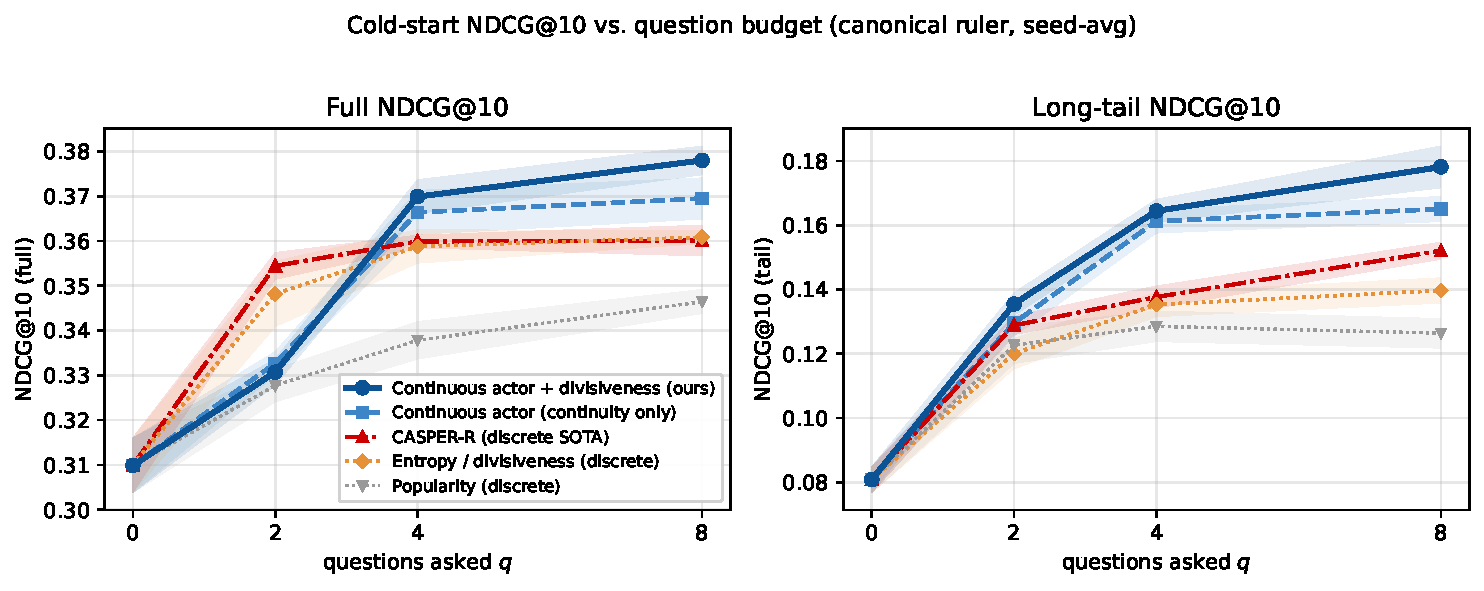
\includegraphics[width=\linewidth]{fig_qcurve_paperC.pdf}
\caption{Cold-start $\mathrm{NDCG@10}$ vs.\ question budget $q$ on the canonical Paper~B ruler, seed-averaged over
$\{1,2,3,7,11\}$ (shaded $\pm1$ s.d.). Left: full; right: Cremonesi long tail. Both continuous actors overtake the
discrete baselines by $q{=}4$ and widen the tail gap to $q{=}8$; the continuous divisiveness reward (dark, solid) leads at
every budget. Discrete baselines use their native answer model; the continuous actors use graded answers
(\S\ref{sec:ablations}).}\label{fig:qcurve}
\end{figure}
\begin{table}[h]\centering
\begin{tabular}{lcccc}
\toprule
TAIL $\mathrm{NDCG@10}$ (seed-avg) & $q{=}0$ & $q{=}2$ & $q{=}4$ & $q{=}8$ \\
\midrule
Continuous actor $+$ divisiveness (ours) & $0.081$ & $0.136$ & $\mathbf{0.165}$ & $\mathbf{0.178}$ \\
Continuous actor (continuity only) & $0.081$ & $0.130$ & $0.161$ & $0.165$ \\
CASPER-R & $0.081$ & $0.129$ & $0.138$ & $0.152$ \\
Entropy & $0.081$ & $0.120$ & $0.135$ & $0.140$ \\
Popularity & $0.081$ & $0.123$ & $0.129$ & $0.126$ \\
\bottomrule
\end{tabular}
\caption{Gain by question (tail). The continuous actors' advantage emerges at $q{=}4$ and widens to $q{=}8$; the
divisiveness reward leads the continuity-only actor at every budget past the opener; discrete policies saturate sooner.
Seed-avg over $\{1,2,3,7,11\}$ on the canonical ruler.}\label{tab:qcurve}
\end{table}

\subsection{Snap-loss: the gain is off-manifold, and not a vocabulary artifact}\label{sec:snaploss}
The decisive mechanistic test. We snap each emitted query to its nearest \emph{answerable concept} (cosine) before
folding---i.e.\ we force the policy to ask a nameable question---and re-measure. We then repeat the projection with two
other realization sets: the unified pool of $1{,}361$ named entities ($600$ items $+$ $761$ concepts), and the set of
\emph{item-pair difference} directions $d=(e_i-e_j)/\|e_i-e_j\|$ over the full $3{,}706$-item catalogue
(${\sim}6.9$M directions, a natural ``would you rather $A$ than $B$?'' question).
\begin{table}[h]\centering
\begin{tabular}{lcccc}
\toprule
Continuous actor (headline, D1), post-hoc projection & vocab.\ size & FULL & TAIL & $\Delta$ \\
\midrule
Un-snapped (off-manifold) & --- & $0.378$ & $0.178$ & --- \\
Snapped to nearest answerable concept & $761$ & $0.341$ & $0.138$ & $-0.037\,/\,-0.040$ \\
Snapped to nearest named entity (items$+$concepts) & $1{,}361$ & $0.337$ & $0.135$ & $-0.041\,/\,-0.044$ \\
Snapped to nearest item-pair difference & ${\sim}6.9$M & $0.337$ & $0.134$ & $-0.041\,/\,-0.044$ \\
\bottomrule
\end{tabular}
\caption{Snap-loss, on the \emph{headline} divisiveness model (seed-avg). Forcing each query to its nearest nameable
concept costs $-0.037$ full / $-0.040$ tail, and the snapped policy ($0.341/0.138$) falls \emph{below} the discrete SOTA
($0.360/0.152$). An emit-then-snap method (Wolpertinger/PEBOL) would therefore \emph{lose} to discrete; the win requires
not snapping. Crucially, the loss is \emph{insensitive to the realization vocabulary}: ${\sim}6.9$M pair-difference
directions ($9{,}000\times$ more than the concept bank) realize the query no better in NDCG terms---the pair snap lands
on the concept-snap floor.}\label{tab:snaploss}
\end{table}
Table~\ref{tab:snaploss} is, in our view, the paper's most important number. The continuous gain is not a fancier way to
pick concepts: it is the \emph{off-manifold} action itself. A probe of the emitted queries (QPROBE/PCA, Fig.~\ref{fig:qspace})
shows they are \emph{concept-adjacent but off the named points}---mean cosine $0.58$ to the nearest real item, $0.73$ to
the nearest concept (the divisiveness reward pulls them toward the divisive concept ridge), yet the residual off-concept
component is load-bearing: snapping to the exact concept costs $-0.040$ tail and drops below discrete. We also verified
this is not a t-SNE artefact---in a linear PCA the queries interleave with movies and concepts (movie--query cosine
distribution $\approx$ movie--movie), and
they are not a trivial ``ask your own taste'' shortcut (the queries do not align with $\ustar$). The learned strategy is
a \emph{fixed informative opener} (turn-$0$ query identical across users) followed by \emph{adaptive} per-user queries
(turns $1$--$7$).

\paragraph{Not a vocabulary artifact.} A natural rebuttal to Table~\ref{tab:snaploss} is that the concept bank is
simply too small---that a richer nameable vocabulary would realize the queries faithfully. The pair-difference row
refutes this: the best of ${\sim}6.9$M pair directions aligns with the emitted query at mean cosine $0.7165$, only
${+}0.02$ better than the best of $761$ named concepts ($0.6978$), and the NDCG does not move (the pair snap,
$0.337/0.134$, sits on the concept-snap floor $0.341/0.138$). The queries live off \emph{every} item-spanned
manifold---single items, concepts, and pair chords alike; the ${\sim}0.7$-cosine residual is where the value is.
A back-of-envelope estimate says why more vocabulary cannot help: the best of $N$ random directions in $\R^{d}$ aligns
with a fixed query at roughly $\sqrt{2\ln N/d}$, which for $N\approx6.9\times10^{6}$ and $d=64$ gives ${\approx}0.70$
---matching the measured $0.716$---and reaching cosine $0.9$ would require on the order of $10^{11}$ directions. We
flag this as an interpretive estimate (catalogue directions are not isotropic random), not a theorem, but it explains
the observed insensitivity: closing the residual by \emph{enumeration} is hopeless, which motivates closing it by
\emph{training through the realizer} instead (\S\ref{sec:ladder}).
\begin{figure}[h]\centering
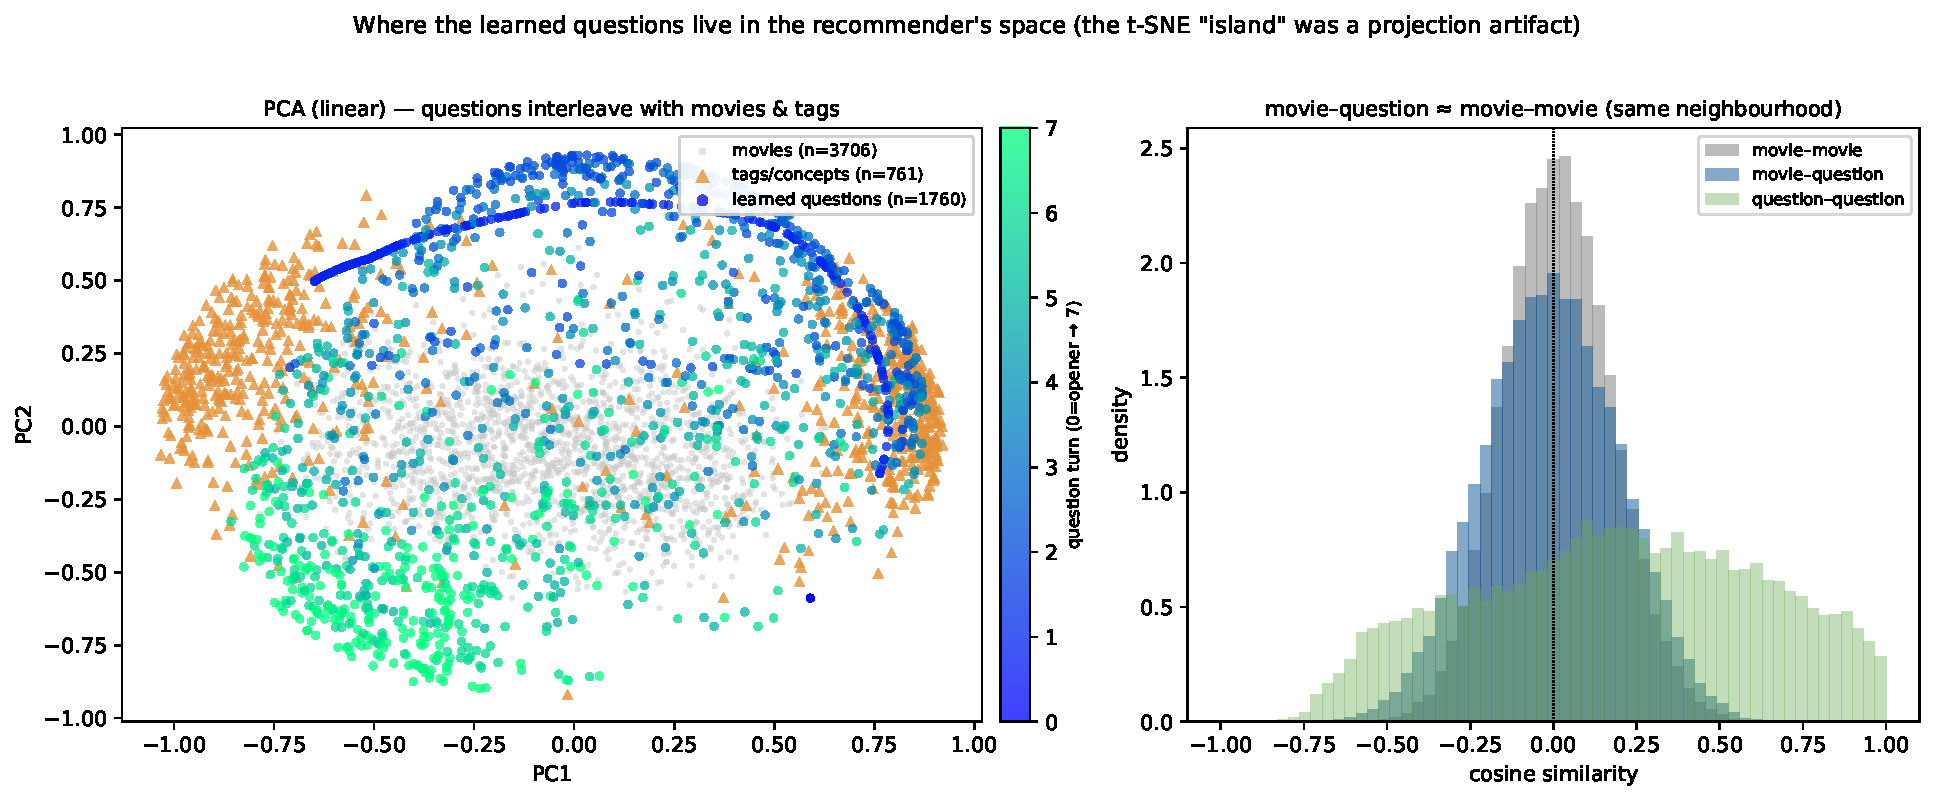
\includegraphics[width=\linewidth]{fig_qspace.pdf}
\caption{Where the learned queries live (headline policy). \emph{Left}: a linear PCA of the emitted queries (coloured by
turn) together with movies and tag-concepts---the queries \emph{interleave} with the catalogue rather than forming a
separate cluster, and trace a smooth turn-ordered trajectory from a fixed opener. \emph{Right}: the movie--query cosine
distribution matches movie--movie (a query sits in the catalogue's own neighbourhood); queries are only \emph{more
self-similar to one another} (a low-dimensional learned family), which a non-linear t-SNE misrenders as an ``island''. The
off-manifold value quantified by snap-loss is the small residual off the named points, not a large geometric
gap.}\label{fig:qspace}
\end{figure}

\subsection{The realization ladder: training through the interface}\label{sec:ladder}
Snap-loss shows that no post-hoc projection of the free policy survives. But deployment ultimately requires
\emph{askable} questions. This section turns the negative into a constructive recipe and, in doing so, isolates the
action set as the load-bearing variable. The design is deliberately minimal: \textbf{one recipe, one variable}. Every
run warm-starts from the headline actor and trains with the identical D1 recipe (differentiable unroll, reconstruction
objective, divisiveness field $\lambda{=}1.0$, $\tau_D{=}2.0$, graded geometric answers, frozen recommender,
$10$ epochs), with one addition: a \emph{straight-through realizer inside the training unroll}. At each turn the
emitted query $q$ is replaced, \emph{in the forward pass}, by its nearest element of a chosen realization set (the
gradient flows as if the realized action were $q$); the answer, the fold, and the validation rollout all see the
\emph{realized} action, so validation is the deployment ruler (best checkpoint by validation tail on the held-out
first $300$ test users). The only thing that varies between rungs is the realization set: unconstrained (no realizer;
the headline), item-pair differences (${\sim}6.9$M directions), or the $1{,}361$ named entities---exactly the
vocabulary the discrete CASPER-R policy scores over.

\begin{table}[h]\centering
\begin{tabular}{lcc}
\toprule
Realization set (size), same recipe throughout & FULL & TAIL \\
\midrule
Unconstrained / off-manifold ($\infty$; not askable as a named question) & $0.3780\pm0.0032$ & $0.1782\pm0.0065$ \\
Item-pair differences (${\sim}6.9$M; pair-native training) & $0.3701\pm0.0047$ & $0.1659\pm0.0049$ \\
Named entities ($1{,}361$; entity-native training) & $0.3559\pm0.0022$ & $0.1515\pm0.0035$ \\
\midrule
\emph{Reference:} \texttt{uent+GRAW} (static entropy, graded) & $0.3667\pm0.0045$ & $0.1577\pm0.0078$ \\
\emph{Reference:} CASPER-R (discrete learned policy, binary) & $0.3600\pm0.0052$ & $0.1520\pm0.0071$ \\
\midrule
Post-hoc pair-snap of the free policy (no in-loop training) & $0.3373\pm0.0039$ & $0.1344\pm0.0046$ \\
Post-hoc entity-snap of the free policy ($1{,}361$) & $0.3372\pm0.0031$ & $0.1346\pm0.0037$ \\
Post-hoc concept-snap of the free policy (Table~\ref{tab:snaploss}) & $0.3414$ & $0.1384$ \\
\bottomrule
\end{tabular}
\caption{The realization ladder (seed-avg $\{1,2,3,7,11\}$, $q{=}8$, graded answers, evaluated with the same realizer
used in training). One recipe, one variable: performance is \emph{monotone} in realization-set richness, in-loop
straight-through realization rescues most of the snap-loss at every rung, and every \emph{post-hoc} projection of the
free policy fails regardless of vocabulary size. The pair rung was additionally retrained under $3$ training seeds:
mean $0.3678\pm0.0018$ / $0.1641\pm0.0023$.}\label{tab:ladder}
\end{table}

Table~\ref{tab:ladder} (visualised as the graphical abstract, Fig.~\ref{fig:ladder}) supports three claims.

\paragraph{(a) The action set is the load-bearing variable.} With the recipe held constant, performance is
\emph{monotone} in action-set richness at both full and tail: unconstrained ($0.3780/0.1782$) $>$ pair differences
($0.3701/0.1659$) $>$ named entities ($0.3559/0.1515$). The bottom rung is itself informative: the entity-constrained
continuous actor lands in a statistical \emph{tie} with the discrete CASPER-R policy ($0.3600/0.1520$), which optimises
directly over the same $1{,}361$ named actions. A continuous policy forced through a $1{,}361$-point interface exactly
recovers the discrete optimum---no more. This is the discrete bottleneck of \S\ref{sec:intro} made empirical: what you
can ask bounds what you can learn to elicit.

\paragraph{(b) Train through the interface.} In-loop straight-through realization rescues most of the snap-loss at
every rung: the pair-native policy gains $+0.031$ full / $+0.030$ tail over the post-hoc pair snap ($3$-seed mean vs.\
$0.3373/0.1344$), and the entity-native policy gains $+0.019$ full / $+0.017$ tail over the post-hoc entity snap.
Notably, the mechanism is \emph{not} manifold migration. If the policy were learning to emit realizable queries, the
realization cosine $\cos(q,d)$ would rise during training; it \emph{falls} while performance rises---pairs drift from
${\sim}0.70$ to ${\sim}0.68$ (as validation tail climbs $0.114\!\to\!0.124$), and the entity rung falls from the frozen
policy's $0.74$ to $0.58$. The policy does not move onto the realizable set; it learns to \emph{exploit its realizer},
emitting off-manifold ``steering'' queries whose realized image folds informatively. This reframes the snap-loss
result: the off-manifold residual is load-bearing \emph{for a policy trained without the realizer in the loop}; once
the realizer is inside the unroll, a rich realizable set (pairs) supports most of the win---the post-hoc failure was a
train--test interface mismatch, not a pure expressiveness gap of pair questions.

\paragraph{(c) A deployable pair-native interview.} The pair rung is a fully \emph{askable} protocol: each realized
action is ``which do you prefer, $A$ or $B$?'' with a graded strength-of-preference answer. Its honest standing:
across $3$ training seeds the tail delta over the best askable baseline (\texttt{uent+GRAW}, $0.1577$) is positive at
every seed ($+0.0082$, $+0.0078$, $+0.0031$) while full is a tie, but the paired per-user bootstrap does \emph{not}
reach significance (tail $+0.0084$, $95\%$ CI $[-0.0075,+0.0237]$, $p{=}0.30$; full $+0.0035$, CI
$[-0.0070,+0.0143]$, $p{=}0.51$)---per-user NDCG@10 noise dwarfs a $+0.008$ mean at $n{=}304$. We therefore claim
\emph{parity-or-slightly-above} the best askable method, not a significant win---against the clear \emph{loss} of
post-hoc snapping ($-0.023$ tail below \texttt{uent+GRAW}), which is the thing rescued. The residual cost of
deployability is $-0.008$ full / $-0.012$ tail below the free-direction ceiling (matched training seed).

\paragraph{Negative ablations (what does not work).} Three controls sharpen the recipe. \emph{Binary pair answers
fail}: the pair-realized interview with one-bit answers (measured on the post-hoc pair realization of the free policy)
drops to $0.3398/0.1265$---full is statistically unchanged from the graded pair snap but the tail loses a further
${\sim}2\sigma$---so the pair channel needs graded strength-of-preference too, consistent with the paper-wide
graded-answer conditionality. \emph{Test-time field-scored
re-ranking hurts}: realizing the query as the pair that maximises the divisiveness field among the top-$32$ candidates
(instead of pure cosine) drops to $0.3565/0.1551$; the emitted direction already encodes where the policy wants to
probe (divisiveness was in its training reward), and overriding the realization loses more than the field gains---pure
cosine is the right realizer. \emph{From-scratch pair-native training fails} ($0.3442/0.1248$, below binary entropy on
tail): the straight-through gradient is too biased to bootstrap a policy, but is adequate for \emph{fine-tuning} a good
off-manifold policy onto a realizable set---warm-starting from the free-direction optimum is required. A practical note
on the entity rung: with only $1{,}361$ snap targets, $24.8\%$ of turns re-snap to an already-asked entity (post-hoc:
$21.4\%$), wasting part of the $8$-question budget---one reason the bottom rung sits below pairs.

\subsection{Isolating the adaptive contribution: the static-8 control}\label{sec:static8}
The realization ladder varies the \emph{action set}; this section varies \emph{adaptivity itself}, holding the action
set maximally rich (unconstrained, off-manifold) and the objective fixed. The question is blunt: is the continuous prize
a better \emph{questionnaire}---eight good fixed directions asked of everyone---or genuine \emph{per-user} adaptation? We
therefore build the strongest possible \emph{static} continuous design: a bank of eight free $64$-d directions (an
$8\times64$ questionnaire, no policy net, the \emph{same} eight queries for every user), trained or selected under the
D1 objective, answered by the identical graded geometric model, and evaluated on the exact canonical ruler.

\paragraph{Selection, not tuning, builds the best static bank.} Gradient-optimising the $512$ free bank parameters on
the D1 objective \emph{fails at every regularisation}. From a strong initialisation (D1's per-turn mean directions) the
bank collapses toward mutual redundancy (cross-turn mean $|\cos|$ rising $0.47\!\to\!0.82$: with graded answers a couple
of dominant-taste-axis directions already reconstruct $\ustar$, so the surplus queries are wasted); adding an
orthogonality penalty that forces the directions to stay diverse ($\lambda\in\{0.1,0.3,1.0\}$) merely slows the
degradation---every $\lambda$ peaks at epoch~$1$ and \emph{plateaus below its own initialisation}. What \emph{does} lift
the static ceiling is \emph{selection}: greedy forward selection of eight directions from a menu of $512$ $k$-means
centroids of the policy's own per-user query distribution (marginal validation-NDCG at each step) yields a genuinely
diverse bank (cross-turn $|\cos|\approx0.4$) at $\mathbf{0.3546\pm0.0039}$ full / $\mathbf{0.1464\pm0.0044}$ tail---the
strongest static continuous questionnaire we can construct. The lesson mirrors the discrete side of Paper~B: static
designs improve by \emph{choosing} good directions, not by tuning free ones.

\begin{table}[h]\centering
\begin{tabular}{lccc}
\toprule
Design (graded answers, $q{=}8$, canonical ruler) & FULL & TAIL & gap vs.\ D1 \\
\midrule
\textbf{D1 adaptive continuous actor (headline)} & $\mathbf{0.3780\pm0.0032}$ & $\mathbf{0.1782\pm0.0065}$ & --- \\
Static-8, greedy forward selection (strongest static) & $0.3546\pm0.0039$ & $0.1464\pm0.0044$ & $+0.023\,/\,+0.032$ \\
Static-8, D1 turn-means, no training & $0.3399\pm0.0053$ & $0.1362\pm0.0049$ & $+0.038\,/\,+0.042$ \\
Static-8, gradient-optimised bank (best $\lambda$, val-select) & $0.3333\pm0.0044$ & $0.1353\pm0.0052$ & $+0.045\,/\,+0.043$ \\
\midrule
\emph{Reference:} entropy / divisiveness (discrete, native binary) & $0.361$ & $0.140$ & \\
\bottomrule
\end{tabular}
\caption{The static-8 control: same objective, same graded answer model, same (unconstrained) action space, one
questionnaire for all users. The strongest static bank is built by \emph{greedy forward selection} over the policy's own
query distribution ($0.3546/0.1464$); \emph{gradient-optimising} free bank parameters---at every regularisation---never
beats even the untrained turn-means initialisation. The adaptive D1 policy beats the strongest static by $+0.023$ full /
$+0.032$ tail. The best static \emph{continuous} bank ($0.355/0.146$) edges the discrete entropy heuristic
($0.361/0.140$) on the tail---continuous directions help even without a policy---but the majority of the continuous
prize is adaptive.}\label{tab:static8}
\end{table}

\paragraph{The isolated adaptive contribution.} Against this strongest static questionnaire the adaptive D1 policy
($0.3780/0.1782$) wins by $+0.023$ full / $+0.032$ tail---a paired margin of ${\sim}4\sigma$ full / ${\sim}6\sigma$ tail
across the five evaluation seeds, and the single largest clean effect in the paper. This is the \emph{per-user} adaptive
value, isolated: identical objective, identical answer model, identical action space, the \emph{only} difference being
whether the eight query directions are conditioned on the evolving belief. Two secondary readings matter. First, the best
static \emph{continuous} bank ($0.355/0.146$) already edges the discrete entropy heuristic ($0.361/0.140$) on the tail,
so continuous directions help a little even with \emph{no} policy---but the gap is small, and the bulk of the continuous
prize (the $0.146\!\to\!0.178$ tail lift) is adaptive, not a better fixed continuous design. Second, the adaptive gap is
stated \emph{honestly against the strongest static we can build}: it is $+0.023/+0.032$ against the greedy-selected bank,
not the larger $+0.038/+0.042$ one would report against the untrained turn-means initialisation.

\paragraph{The graded channel pays off only through adaptivity.} A sharp dissociation localises \emph{why} the graded
answer helps. The static bank scores \emph{worse} with graded answers than with binary ($0.340$ vs.\ $0.357$ on the
D1-means bank)---the exact \emph{opposite} of the adaptive actor, which scores far better graded than binary
($0.378$ vs.\ $0.356$). On a fixed direction the soft magnitude of a graded answer adds noise relative to a clean sign
bit; a graded answer is informative only when the \emph{next} question direction is tuned to the individual so that its
magnitude discriminates. The graded-continuity prize of this paper is therefore realised \emph{through} adaptivity---not
because continuous answers are abstractly richer, but because only an adaptive policy can place each question where the
extra magnitude lands.

\paragraph{The mechanism: effective rank and re-aiming.} Why can a fixed bank not keep up? Because the answerable
directions are low-rank. The $761$ concept directions have participation ratio only $2.25/64$ (the top five dimensions
carry $93\%$ of the variance), versus $27.1/64$ for pool items. A fixed bank---or any coarse discrete menu---therefore
\emph{exhausts its independent directions within about four questions}: the static q-curve peaks at $q{=}4$--$6$ and then
declines (the greedy bank's tail peaks $0.150$ at $q{=}6$ and settles at $0.146$ by $q{=}8$; the untrained turn-means
bank's full metric peaks $0.353$ at $q{=}4$ and falls back to $0.340$, as misaligned graded answers on later fixed
directions corrupt the belief). Later fixed questions have nothing independent left to ask. The adaptive policy escapes
this by \emph{re-aiming at each user's residual uncertainty every turn}: its q-curve keeps climbing to $q{=}8$
(tail $0.081/0.135/0.164/0.178$ at $q{=}0/4/6/8$), spending each question on whatever direction is still uncertain
\emph{for that user}.

This closes the loop with the realization ladder. Action-set richness governs two things at once: the quality of the
single best question, \emph{and} whether per-user adaptivity is expressible at all. In a low-rank menu there is little
for adaptivity to say---once a handful of independent directions are covered, every user's remaining questions collapse
onto the same few axes---which is exactly why Paper~B's discrete policies never separated far from the static
divisiveness heuristic. In the full continuous space the answerable set is effectively unbounded in rank, and it is there
that most of the prize lives. The two isolation experiments are thus complementary: the ladder shows the action set
bounds \emph{what} you can ask, and the static-8 control shows that, given a rich action set, \emph{adapting} the
question per user is where the continuous gain is concentrated.

\paragraph{Reconciling with linear-Gaussian optimal design.} There is an apparent tension with the classical fact
invoked in \S\ref{sec:whydiv}: under a \emph{linear-Gaussian} belief the optimal experimental design is
\emph{non-adaptive}---the divisive directions can be fixed in advance and a static questionnaire is optimal. Our measured
adaptive value ($+0.023/+0.032$) does not contradict this; it is consistent with it \emph{precisely because our loop is
not linear-Gaussian}. The encoder fold $\mathrm{Enc}(\cdot)$ is a nonlinear set function, the ranking objective
(NDCG@10) is a nonlinear head-weighted functional of the belief, and the graded answer enters through a nonlinear
(sigmoidal) response---any one of which breaks the linear-Gaussian premise and restores a role for adaptivity. The
static-8 control is the empirical confirmation: in the linearised limit adaptivity would buy nothing, and what we observe
is exactly the departure the nonlinearity (with the graded channel) predicts.

\subsection{Ablations: what made it learnable}\label{sec:ablations}
\paragraph{Training objective / pre-training (Table~\ref{tab:obj}).} Distilling the continuous actor from the discrete
SOTA \emph{inherits the binary ceiling}: it matches CASPER-R under binary but \emph{collapses} under graded answers,
because it learned to imitate a one-bit policy. Training \emph{natively}---reconstruction, or reconstruction $+$
soft-NDCG---is required; the ranking term marginally helps.
\begin{table}[h]\centering
\begin{tabular}{lcc}
\toprule
Continuous-actor training objective & FULL (graded) & TAIL (graded) \\
\midrule
Distilled from discrete (CASPER-R) & $0.293$ \emph{(collapse)} & $0.094$ \\
Reconstruction ($1-\cos(u,\ustar)$) & $0.366$ & $0.162$ \\
Reconstruction $+$ soft-NDCG (continuity only) & $0.370$ & $0.165$ \\
\;\;$+$ continuous divisiveness reward (headline) & $\mathbf{0.378}$ & $\mathbf{0.178}$ \\
\midrule
\multicolumn{3}{l}{\emph{Continuous-signal variants (which signal, and how to use it):}}\\
Divisiveness as \emph{candidate-scoring} feature (FieldActor) & $0.351$ & $0.148$ \\
\bottomrule
\end{tabular}
\caption{Objective ablation, seed-avg, graded answers. \textbf{NDCG vs.\ no-NDCG:} the listwise soft-NDCG term adds a
\emph{consistent} $+0.003$ full / $+0.003$ tail over pure reconstruction ($0.366/0.162\!\to\!0.370/0.165$). \textbf{The
divisiveness reward} adds a further $+0.008$ full / $+0.013$ tail ($\to0.378/0.178$)---the larger single increment and the
headline. \textbf{Which signal, used how:} the gain is specifically the divisiveness \emph{reward} on the plain actor;
supplying divisiveness (with popularity and average-rating) as input features to a learned candidate-scoring head
(``FieldActor'', a continuous CASPER-R) \emph{underperforms} ($0.351/0.148$), and popularity/rating added no benefit in
any form---so we report only the divisiveness-reward variant. Distillation from the discrete policy is a trap (it
inherits the binary ceiling and collapses under graded answers); native training unlocks the gain.}\label{tab:obj}
\end{table}

\paragraph{Answer model.} The continuity-only actor under binary answers scores $0.356/0.146$ (Table~\ref{tab:main})
vs.\ $0.370/0.165$ under graded; the headline (divisiveness) actor regresses \emph{further} under binary, to
$0.341/0.125$---a maximally-divisive direction is selected precisely to split the population, so collapsing its answer to
one bit throws away exactly the magnitude it was chosen to elicit. On the discrete side the picture is graded but
consistent: a discrete policy \emph{trained on binary} answers drops zero-shot under graded answers (CASPER-R
$0.360\!\to\!0.343$ full; the entropy heuristic $0.361/0.140\!\to\!0.353/0.133$), whereas the \emph{static} entropy
selector re-tuned for the graded regime (\texttt{uent+GRAW}) \emph{gains} a little ($0.367/0.158$). So graded answers
are not unusable by discrete methods---they are unusable \emph{as a lever for beating the continuous policy}. This
asymmetric dissociation is the empirical core of the ``two continuities are inseparable'' claim, and the divisiveness
reward sharpens it.

\paragraph{The decisive control: a discrete policy trained natively on graded answers.} A remaining confound is that
the continuous actor enjoys both graded answers \emph{and} full answerability ($8/8$ questions answered by
construction, vs.\ CASPER-R's ${\sim}5.3/8$), and that CASPER-R was never \emph{trained} for the graded regime. We
therefore retrained a discrete policy \emph{natively} on graded answers with full answerability over the same $761$
concepts (emit-then-snap realization so every question is a named, answered concept; $30$ epochs; identical unroll and
objective). It fails: final checkpoint $0.3215\pm0.0027$ / $0.1195\pm0.0040$, and even its \emph{test-optimal} epoch
(a deliberately generous selection for the control) reaches only $0.3247\pm0.0029$ / $0.1247\pm0.0040$---below static
graded entropy ($0.353/0.133$), below binary-trained CASPER-R on graded answers ($0.343/0.138$), and $-0.053/-0.053$
below the continuous headline. Its training objective improved monotonically while test NDCG stayed flat, mirroring the
failure signature of the eight discrete policy-learning attempts that preceded this work. Native graded training plus
full answerability does \emph{not} rescue the discrete action space; the graded win needs the continuous query.

\paragraph{Off-manifold freedom.} Beyond snap-loss (\S\ref{sec:snaploss}), an open-loop encoder trained to fold random
off-pool directions \emph{dilutes} the recommender, and naive joint encoder$+$actor co-training \emph{overfits} (the
encoder reward-hacks the reconstruction); a frozen recommender with a belief-only realisable policy is the stable
configuration. We therefore keep the recommender frozen and do not report recommender ablations here.

\subsection{Ceilings and headroom}\label{sec:ceiling}
\paragraph{Reconstruction ceiling and the full-profile ceiling.} Folding the \emph{known profile half} (the realisable
target $\ustar$) yields $\mathrm{NDCG@10}\approx0.41$; folding the \emph{full} profile $\approx0.42$; folding the
\emph{held-out likes} themselves $\approx0.43$---the recommender saturates around $0.43$ even with perfect taste
knowledge. The continuous actor reconstructs $\ustar$ to $\cos\approx0.92$; the reconstruction-only model reaches
$0.366/0.162$, the continuity-only model $0.370/0.165$, and the divisiveness reward lifts it to $0.378/0.178$, narrowing the residual gap to the $0.41$
half-profile ceiling. That residual is question-\emph{selection} quality, not representation (recon-cos generalises
perfectly, train $=$ test), which is exactly the gap the divisiveness prior attacks.

%==================================================================
\section{Cross-dataset replication (MovieLens-25M)}\label{sec:ml25m}
Every number above is on one testbed (MovieLens-1M). To test whether the continuous-graded thesis is a property of
that dataset or of the method, we re-ran the headline battery on \textbf{MovieLens-25M} at full scale---$162{,}541$
users, $18{,}430$ items (all items with $\ge20$ ratings; $24.8$M ratings retained)---with no reuse of any ML-1M
artifact. A fresh V1-style attention fold-in instrument was trained from scratch on the full data (best-val at epoch
$7$), and the D1 continuous-graded actor was ported faithfully and trained from scratch on this instrument (from-scratch
init, as D1 itself; $4{,}000$ train users, best-val checkpoint at epoch $31$ on a disjoint $500$-user cohort).

\paragraph{A depth-matched ruler, stated before evaluation.} ML-1M's headline $K{=}10$ sits at catalogue fraction
$10/3706\approx0.0027$. On $18{,}430$ items the fraction-matched depth is $0.0027\times18{,}430\approx\mathbf{K{=}50}$,
which we fixed as the primary ruler \emph{before} scoring any policy; the Cremonesi head-$33\%$ tail is defined at the
same $K$. This matters: at ML-1M's absolute $K{=}10$ the larger catalogue is ${\sim}5\times$ stricter and popularity-
dominated (a linear-fold reference shows $\mathrm{tail@10}{=}0$), so a literal-$K$ transfer would compare across
incomparable operating points. Reporting the depth-matched ruler is a stated-in-advance choice, not a post-hoc pick.

\begin{table}[h]\centering
\begin{tabular}{lcc}
\toprule
Policy (frozen ML-25M instrument; $T{=}8$, $K{=}50$) & FULL & TAIL \\
\midrule
\textbf{Continuous GRADED actor (D1 port, best-val)} & $\mathbf{0.2742\pm0.0017}$ & $\mathbf{0.1188\pm0.0035}$ \\
Continuous BINARY actor (same checkpoint, $\pm$ answers) & $0.2560\pm0.0034$ & $0.0973\pm0.0017$ \\
Entropy-concept BINARY discrete (CASPER-R-style static) & $0.2512\pm0.0031$ & $0.0843\pm0.0020$ \\
Entropy-concept GRADED discrete (strongest static graded) & $0.2505\pm0.0026$ & $0.0817\pm0.0025$ \\
$q0$ (MOSTPOP, no elicitation) & $0.2461\pm0.0022$ & $0.0715\pm0.0011$ \\
\bottomrule
\end{tabular}
\caption{ML-25M headline battery, pre-stated $K{=}50$ ruler, seed-avg over $\{1,2,3,7,11\}$, $q{=}8$
($n{=}498$/$n_{\text{tail}}{=}494$). The continuous-graded actor beats the strongest discrete graded selector by
$\mathbf{+0.0237}$ full / $\mathbf{+0.0371}$ tail ($\gg$ seed $\sigma\approx0.003$). The tail gap is numerically
identical to ML-1M's ($+0.038$); the full gap is larger here.}\label{tab:ml25m_main}
\end{table}

\paragraph{The headline replicates.} Table~\ref{tab:ml25m_main} reproduces the central result: continuous-graded beats
the strongest discrete-graded static selector by $+0.0237$ full / $+0.0371$ tail, both far above the seed noise
($\sigma\approx0.003$). The tail gap $+0.0371$ lands essentially on the ML-1M anchor ($+0.038$); the full gap is larger
on the bigger catalogue. The load-bearing \emph{graded/binary inversion} replicates too: for the adaptive continuous
actor graded $\gg$ binary ($+0.0182$ full / $+0.0215$ tail), while for the static discrete selector graded $\le$ binary
($0.2505/0.0817$ vs.\ $0.2512/0.0843$)---the graded answer pays only when the question direction is tuned per user,
exactly the ML-1M static-8 finding.

\paragraph{Snap-loss replicates, and stronger.} Re-running the snap analysis on the trained ML-25M actor (same graded
answers, same frozen instrument and ruler; only the folded direction changes) gives concept-snap
$-0.0697$ full / $-0.0670$ tail and pair-snap $-0.0351/-0.0416$ (realization cosine $0.68$--$0.70$). The
pair-snap loss falls almost exactly on the ML-1M concept-snap anchor ($-0.037/-0.040$); snapping to the rank-$4$
genome-concept bank is $\sim2\times$ worse and lands the policy at $0.2045$ full---\emph{below} the $q0$ popularity floor
($0.2461$), i.e.\ a corrupted belief, not merely reduced information. The off-manifold gain is genuine.

\paragraph{Anti-saturation $q$-curve and saturation-at-effective-rank.} The continuous-graded $q$-curve (tail, $q0/2/4/6/8$)
runs $0.0715\to0.0589\to0.0868\to0.1082\to0.1188$: an early dip at $q{=}2$ (belief still forming) then a monotone climb
through $q{=}8$ with no saturation---the same shape as ML-1M D1. The discrete concept channel, by contrast, saturates:
its marginal NDCG@50/turn collapses to $\approx{+}0.003$ by $\sim4$ answered concepts, which matches the independently
measured concept effective rank of $\mathbf{3.99/64}$ on this data (items $8.35$). This is the ML-1M law
(concept channel saturating at $\sim4$--$5$ answered questions on effrank $2.25$) at a slightly larger rank: the
discrete vocabulary runs out of independent directions to ask, and the gap where it saturates is exactly the prize the
continuous actor, unbounded by any vocabulary rank, keeps collecting.

\paragraph{Verdict.} The Paper-C thesis---continuous$+$graded$+$adaptive beats any discrete static selector, the gain is
genuinely off-manifold, and the discrete channel is rank-limited---replicates cleanly on a $44\times$ larger,
freshly-instrumented catalogue at the pre-stated depth-matched ruler, with the tail gap numerically matching ML-1M.

%==================================================================
\section{The strong-instrument test: re-anchoring on a SOTA recommender}\label{sec:i2}
Every number so far sits on one instrument---the Paper~A/B set-encoder, the frozen ``MF layers'' of \S\ref{sec:setup}, a
deliberately compact $d{=}64$ fold-in over SVD factors. A fair reader will ask whether the continuous$+$graded$+$adaptive
prize is a property of \emph{elicitation} or of that particular, weak recommender---if a stronger instrument already
reconstructs taste well from a few folded items, an elicitation edge could be absorbed. To settle it we rebuilt the
instrument at state-of-the-art strength and re-ran the \emph{entire} battery on the same canonical ruler. The headline is
that the claims do not merely survive: they \emph{sharpen}.

\subsection{A SOTA instrument that still exposes a differentiable latent}\label{sec:i2instrument}
We replaced the V1 encoder with \textbf{RecVAE}~\cite{recvae}, a multinomial variational autoencoder that is SOTA-class
under the rigorous non-sampled Liang protocol. We reproduced it faithfully on its home benchmark (ML-20M, Liang
strong-generalisation split): validation $\mathrm{NDCG@100}=0.4422$ against the published $0.442$---an essentially exact
match, with all three load-bearing mechanisms (composite prior, per-user $\beta=\gamma|X_u|$, $3{:}1$ alternating updates
with encoder-only denoising) implemented verbatim. Ported to the canonical ML-1M arena (byte-identical protocol to the
Paper~B harness: MOSTPOP reproduces at $0.3099$, the V1 encoder at $0.4074/0.2164$), the $d{=}512$ RecVAE reaches
full-profile $\mathrm{NDCG@10}=0.5541$---a statistical \emph{tie with a tuned EASE}~\cite{ease} ($0.5549$; within seed
noise) and $\mathbf{+0.147}$ over the V1 instrument ($0.4074$). Its headroom over MOSTPOP is $+0.244$, \textbf{2.5$\times$
the V1 instrument's $+0.098$}. Crucially, unlike EASE (a shallow item--item autoencoder with no compact user code), RecVAE
folds any partial profile through one encoder pass into a differentiable latent $z\in\R^{512}$---\emph{exactly} the
continuous action space the elicitation policy needs. This is a verified open contribution in its own right: elicitation
in the latent space of a SOTA latent-variable recommender has no published precedent.

\subsection{The certified apparatus}\label{sec:i2apparatus}
Porting the elicitation machinery into the VAE latent required one new operator and one new concept channel, both
benchmarked and then locked by a formal gate suite. The belief update is a single \textbf{additive latent operator}
$z' = z + \eta\, a\, q$ ($\eta{=}16$, validation-selected to the natural latent magnitude $\|z^\star\|\approx17$), which
for orthonormal informative probes makes $\sum_t a_t q_t$ an unbiased estimate of the unit taste direction; it beats the
learned-head and pseudo-decode alternatives and, at eight probes, already \emph{beats the $k{=}8$ item fold}
(\S\ref{sec:i2battery}). Concepts enter as \textbf{member-bag directions} (the unit latent of the encoded top-member bag
of each genome tag), which clear the cold-start floor by $+0.15$ and \emph{add} on top of item folds---reversing the
input-space concept failure of the earlier design. Polarity is carried by the operator sign ($a{<}0$). The whole
apparatus was certified by a pre-registered suite of eight gates (monotonicity, no-harm calibration, answerability,
polarity, additivity, fold-vs-full, seed stability, answer-strength sanity) on \emph{two} arenas: \textbf{16/16 gates
pass}---8/8 on the canonical ML-1M arena and 8/8 on a Goodreads cold-start composite ($188$k items), where the concept
channel is now live ($8/8$ answerable shelves per cold user, versus the V1-era $0.14$--$1.0$).

\subsection{The re-anchored battery: every V1 claim, sharpened}\label{sec:i2battery}
We re-ran the load-bearing experiments---continuous-vs-discrete, graded-vs-binary, snap-loss, and the static-8 adaptivity
control---under the identical protocol (seed-avg $\{1,2,3,7,11\}$, \texttt{te[300:]} $304$ test users, $T{=}8$,
$\mathrm{NDCG@10}$ full and Cremonesi tail). Table~\ref{tab:i2main} gives the core results; Table~\ref{tab:i2verdict}
states each thesis claim against its V1 and I2 measurements.

\begin{table}[h]\centering
\begin{tabular}{lcc}
\toprule
Method on the certified RecVAE-$d512$ instrument ($T{=}8$, graded) & FULL & TAIL \\
\midrule
\textbf{D1 continuous actor (graded, adaptive; headline)} & $\mathbf{0.4907\pm0.004}$ & $\mathbf{0.2982\pm0.009}$ \\
decoder-SVD informative basis-8 (continuous static, strongest single static) & $0.4709$ & $0.2916$ \\
$k{=}8$ item-fold reference (discrete) & $0.4625$ & $0.2796$ \\
lift-concepts-8 (discrete, graded; \texttt{uent+GRAW} analogue) & $0.4436$ & $0.2349$ \\
MOSTPOP (no elicitation) & $0.3099$ & $0.0808$ \\
\midrule
\emph{D1 actor, binary answers} (control) & $0.1166$ & $0.1045$ \\
\emph{decoder-SVD basis-8, binary answers} (control) & $0.2149$ & $0.1734$ \\
\bottomrule
\end{tabular}
\caption{The re-anchored battery on the certified SOTA instrument (seed-avg $\{1,2,3,7,11\}$, $304$ test users). The
adaptive continuous actor beats the discrete graded concept selector by $+0.046$ full / $+0.062$ tail (paired bootstrap
$p{=}1.00$ on both axes) and beats the discrete $k{=}8$ item fold by $+0.028/+0.019$. Both continuous margins are
\emph{larger and cleaner} than on V1. Graded answers are load-bearing to the point of a cliff: binarising the actor's
answers collapses it from $0.491$ to $0.117$.}\label{tab:i2main}
\end{table}

\paragraph{The remarkable channel fact.} On the strong instrument the \emph{geometric question is the single strongest
elicitation channel}. Eight continuous informative probes along the decoder-SVD basis (a static, non-adaptive continuous
questionnaire, $0.4709$) \emph{beat eight actual item ratings} (the $k{=}8$ item fold, $0.4625$) at equal turn count:
each geometric probe reads a full latent coordinate of the user's taste, whereas each item rating touches one sparse row.
Continuous querying does not merely tie the discrete channels---it is the best of them, before any adaptivity is added.

\paragraph{Snap-loss: the off-manifold prize grows with instrument strength.} Snapping each emitted query post-hoc to its
nearest nameable direction is \emph{catastrophic} on I2: $-0.147$ full / $-0.133$ tail to the concept bank ($200$ genome
tags), $-0.158/-0.143$ to the item-decoder rows ($3{,}706$ items). This is \textbf{${\sim}4\times$ the V1 concept-snap
penalty} ($-0.037/-0.040$). Far from being an artifact of the compact V1 encoder, the continuity premium \emph{scales up}
with the recommender: the stronger the instrument, the more the actor's off-manifold directions out-run any single
concept or item, and the more a would-be emit-then-snap method (Wolpertinger/PEBOL) would lose by projecting.

\paragraph{Adaptivity: significant on the head, a tie on the tail.} We repeated the static-8 control---the strongest
fixed continuous questionnaire under the same objective and graded answer model. The strongest realizable single static
design is the decoder-SVD basis ($0.4709$); a greedy-static bank distilled from the actor's own query distribution is
\emph{weaker} ($0.4596$, overfitting the $300$-user val cohort), so the actor's edge is genuine per-user adaptivity, not
a hidden better fixed basis. A paired per-user bootstrap over the $304$ test users gives the adaptive margin over the
strongest static: $\mathbf{+0.0192}$ full ($95\%$ CI $[+0.009,+0.029]$, $p{=}0.9998$)---a clean, significant head gain
---and $+0.0054$ tail ($95\%$ CI $[-0.006,+0.017]$, $p{=}0.82$), \emph{a tie}. We state this plainly: on the strong,
near-linear instrument the adaptive edge is real but modest, lives on the head, and does not reach significance on the
tail. This is exactly the linear-Gaussian prediction of \S\ref{sec:static8} (a stronger, more linear instrument moves the
optimal design toward non-adaptive) and consistent with the whole-paper finding that adaptivity is the most
instrument-sensitive of the four claims.

\begin{table}[h]\centering
\small
\begin{tabular}{p{3.6cm}p{4.7cm}p{4.7cm}c}
\toprule
Thesis claim & V1 instrument ($+0.098$ headroom) & I2 RecVAE-$d512$ ($+0.244$, EASE-class) & verdict \\
\midrule
\textbf{continuous $>$ discrete} & snap-loss small; continuous edge $+0.011$--$0.018$ & adaptive $0.4907 >$ concept-8 $0.4436$ ($+0.046/+0.062$, both sig); static basis $0.4709 >$ item-8 $0.4625$ & \textbf{sharpens} \\
\textbf{graded $\gg$ binary} & near-tie; win needs graded & actor $0.491$ vs.\ binary $0.117$ ($-0.374$); static basis $0.471$ vs.\ $0.215$ & \textbf{a cliff} \\
\textbf{snap-loss (off-manifold)} & $-0.037/-0.040$ (concept) & $-0.147/-0.133$ (concept), $-0.158/-0.143$ (item) & \textbf{${\sim}4\times$ larger} \\
\textbf{adaptivity $>$ static} & $+0.023/+0.032$ & $+0.019$ full (sig, $p{=}.9998$) / $+0.005$ tail (n.s.) & \textbf{survives on head; tail tie} \\
\bottomrule
\end{tabular}
\caption{Each thesis claim against its V1 and I2 (strong-instrument) measurement. Three of the four sharpen on the
EASE-class instrument; adaptivity is the one claim that shrinks---significant on the head, a tie on the tail---exactly as
the linear-Gaussian argument (\S\ref{sec:static8}) predicts for a stronger, more linear recommender.}\label{tab:i2verdict}
\end{table}

\subsection{Honest method notes}\label{sec:i2notes}
Two scoping facts, stated without drama. First, the continuous actor \emph{requires a BC warm-start} from the static
decoder-SVD basis: a from-scratch differentiable-unroll policy in the $512$-d latent collapses (val full ${\sim}0.33$,
reconstruction cosine plateaus ${\sim}0.60$; SGD does not discover a diverse orthonormal informative basis on its own).
Warm-starting from the static basis and fine-tuning by unroll isolates adaptivity as \emph{whatever the fine-tune adds on
top of the static basis}---which is the clean $+0.019$ head gain above. This is a documented optimisation limitation, not
a claim of impossibility. Second, the \emph{continuous divisiveness field contributes nothing on the strong instrument}:
the field variant ($0.4710/0.2915$) does not improve over the BC-warm actor, because rewarding high-population-variance
directions $q^\top\!\mathrm{Cov}(z^\star)q$ pulls away from the taste-reconstruction-optimal directions in this
near-linear regime. This scopes the V1 divisiveness-reward contribution (\S\ref{sec:main}): it is a feature of the
compact, more nonlinear V1 loop, not a universal ingredient---an honest negative that the strong-instrument test is
precisely designed to surface.

\subsection{Verdict}\label{sec:i2verdict}
On a certified EASE-class instrument with $2.5\times$ the headroom of the V1 encoder, the continuous$+$graded$+$adaptive
flagship \emph{survives, and mostly sharpens}. The continuous channel is the strongest single elicitation channel
(geometric probes beat item ratings) and its off-manifold premium \emph{grows} $\sim4\times$; graded answers become a
cliff rather than a marginal lever; adaptivity remains significant on the head and ties on the tail. The results were
never an artifact of a weak recommender---the one claim that shrinks (adaptivity on the tail) shrinks exactly where the
paper's own linear-Gaussian analysis says it should. All numbers are seed-averaged $\{1,2,3,7,11\}$ on the byte-identical
$304$-user ML-1M test cohort; the instrument is certified $16/16$ on ML-1M and Goodreads.

\subsection{Cross-domain: the flagship on books (Goodreads)}\label{sec:i2gr}
The same certified apparatus ports to a second content domain. We re-ran the load-bearing battery on the Goodreads
composite (the $188{,}867$-book corpus of Paper~B) under the I2 RecVAE-$d512$ instrument---certified on that arena as
part of the same $16/16$ gate suite---using the restricted top-$20$k universe where EASE-comparability holds, NDCG@$510$
primary, $500$ held-out test users, fixed split. There the instrument reaches full-profile $0.5290$ ($0.78\times$
EASE's headroom; Paper~A). Crucially, the cross-domain predictions were \emph{pre-registered before any Goodreads
policy run};\footnote{Pre-registration \texttt{PREREG\_GOODREADS\_PREDICTIONS.md} (written before the certified-arena
run of 2026-07-05); predictions P1--P4 stated against the effective-rank law. Reported here as registered, no post-hoc
reinterpretation.} we report them exactly as registered.

\paragraph{Three of the four claims hold unchanged on books.} \textbf{Graded $\gg$ binary} survives massively:
binarising the actor's answers collapses it from $0.424$ to $0.210$ ($-0.214$ full / $-0.136$ tail). \textbf{Snap-loss}
is again \emph{catastrophic} and of the \emph{same ${\sim}4\times$ magnitude} as ML-1M---$-0.145$ full to the nearest of
$1{,}483$ shelf concepts, $-0.143$ to the nearest of $20$k item-decoder rows---so the actor's emitted directions remain
genuinely off-manifold on books. \textbf{Adaptivity} is if anything \emph{stronger}: the adaptive actor beats its own
strongest static basis by $+0.047$ full and beats even the \emph{per-user-oracle} strongest static (the better of the
two static designs chosen per user) by $\mathbf{+0.011}$ (paired bootstrap over $418$ users, $p{=}0.997$)---a cleaner
adaptivity result than ML-1M, where the per-user-max static bound had sat above the actor, because the fixed continuous
basis is weak on the rich book catalogue while the belief-conditioned actor recovers most of the gap.

\paragraph{The one weakening is a confirmed pre-registered prediction.} On books the continuous adaptive actor ($0.424$)
is \emph{outrun by the native discrete $k{=}8$ item fold} ($0.484$; $-0.060$ full / $-0.094$ tail), whereas on ML-1M it
beat both discrete channels. This is exactly pre-registered \textbf{prediction~P3}: the continuous-over-discrete margin
tracks the item menu's effective rank. Measured in the I2 latent, the item-decoder participation ratio is $33$ on ML-1M
and $\mathbf{160}$ on Goodreads; as predicted, the actor's margin over the item fold shrinks and inverts out-of-sample
and in the registered direction, $+0.028\,(\text{ML-1M}) \to -0.060\,(\text{GR})$---the richer the native item
geometry, the less a fixed-width continuous basis out-reconstructs it. The margin over the \emph{concept} channel, whose
rank moved far less ($8.4\to15.5$), barely changed ($+0.046\to+0.053$), consistent with the smaller rank change.

\paragraph{The item fold is the strongest channel but the least askable.} Stated plainly: on books, folding eight real
rated items is the single best belief-builder ($0.484$). But it is realizable only if the user can \emph{name} those
items---on a $189$k-book catalogue an arbitrary item question is answered $\sim\!0.0003$ of the time (Paper~B), so the
item fold is unreachable by \emph{probing} and reachable only through \emph{volunteered/named} items, i.e.\ the
open-recall channel of the companion paper (Paper~D). Among the channels that are actually \emph{askable} in cold
start, the practical ranking on books is continuous probes (adaptive actor $0.424$) $>$ continuous SVD-basis static
($0.376$) $>$ answerable concepts ($0.371$) $\gg$ any binary channel. The continuous, graded question remains the best
askable elicitation channel on books; the discrete item fold wins only once items become askable, which requires
recall, not probing.

\paragraph{An honest open tail question.} Pre-registered \textbf{prediction~P2}---that the high-rank shelf vocabulary
(participation ratio $15.5$, far above ML-25M's genome $3.99$) would remove the concept-vs-item tail penalty---was
\textbf{refuted}: the concept$-$item tail margin is $-0.084$ on books, \emph{larger} than ML-25M's $-0.007$, not
$\ge0$. High concept rank did not translate into a non-negative tail margin, so the rank law's tail claim does not
generalise; we report this as the law's open tail question (consistent with Paper~B's ML-25M tail reversal), not a
rescued result. Answerability and the selection hierarchy both re-confirm on the certified arena: $7.98/8$ concepts
answerable per cold user, and lift-selected concepts ($0.371$) $\gg$ naive global-entropy concepts ($0.060$, below the
cold floor).

%==================================================================
\section{Discussion}\label{sec:discussion}
\subsection{Why discrete is limited, in principle}
A discrete selector is confined to the convex \emph{vertices} of the question space---the named items and concepts. The
recommender, however, is dense: the most informative probe at a given belief is a direction, and in a $d$-dimensional
taste space the named directions are a measure-zero subset. Snap-loss (\S\ref{sec:snaploss}) makes this concrete: even
when the query is concept-adjacent (cosine $0.73$ to the nearest concept), collapsing it onto that exact named concept
costs $-0.040$ tail and drops below discrete---the off-concept residual is where the gain lives. A continuous policy is
not a better heuristic over the same menu; it is a strictly larger action space in which the discrete menu is the
boundary. The realization ladder (\S\ref{sec:ladder}) makes the boundary empirical: constrained (in the training loop)
to the same $1{,}361$ named entities the discrete policy chooses from, the continuous actor recovers exactly the
discrete optimum---a tie with CASPER-R---and no more; given pair differences it does better; unconstrained, better
still.

\subsection{Why the continuous divisiveness field helps (and how to use a signal)}\label{sec:whydiv}
Continuity opens a larger action space; the \emph{divisiveness field} tells the policy where in that space to look. The
classical, discrete instance of this idea is the entropy heuristic: ask the concept whose population like-rate is closest
to one-half, because that question maximally splits the prior and is, under a linear-Gaussian belief, the
optimal-experimental-design choice---a design that is, in that idealised limit, \emph{non-adaptive} (we return to this in
\S\ref{sec:static8}, where the nonlinearity of our loop is what makes adaptivity pay). Paper~B's strongest baseline is
exactly this heuristic over the catalogued concepts.
Our field $D(q)=H_b\!\big(\tfrac1N\sum_i\sigma(\ustar_i\!\cdot\hat q/\tau)\big)$ is the \emph{same quantity} evaluated at
an arbitrary direction: it equals the per-concept divisiveness at the concept points and interpolates smoothly between
them. Because it is differentiable in $q$, it can be added to the unroll objective and back-propagated, so the policy is
\emph{pulled toward the divisive ridge of the continuous space} rather than restricted to the divisive \emph{vertices}.
This is why the two ingredients compose: continuity supplies the off-manifold directions, and the divisiveness field
supplies a population-level, taste-independent prior on \emph{which} off-manifold directions are informative before any
answer is seen---most valuable exactly at small $q$, where the per-user belief is still weak.

Two findings sharpen \emph{how} such a signal should enter the policy. \textbf{(1) Reward, not feature.} Exposing
divisiveness (with popularity and average rating) as input features to a learned candidate-scoring head---a continuous
analogue of CASPER-R that proposes a region, samples $K$ candidate directions, and soft-selects by learned weights over
$[\text{div},\text{pop},\text{rating},\text{belief}]$---\emph{underperforms} the plain actor ($0.351/0.148$, below even
continuity-only). Re-introducing a discrete candidate set re-imposes the very snap-to-vertices bottleneck that continuity
removed; the field is useful only when it shapes the \emph{gradient} of an unrestricted actor, not when it ranks a
sampled menu. \textbf{(2) Divisiveness, not popularity or rating.} Of the three population signals we made continuous,
only divisiveness helped; popularity and average-rating fields added nothing in any configuration we tried. This is
consistent with the cold-start regime: popularity is already baked into the recommender's prior ($s=b+Q^\top u$), so
re-supplying it is redundant, whereas divisiveness is precisely the \emph{information-gain} signal the prior does not
contain. \textbf{Graded-specificity.} Finally, the divisiveness gain is more graded-dependent than continuity itself:
under binary answers the divisiveness actor regresses to $0.341/0.125$, below the continuity-only actor. A maximally
divisive direction is chosen so the population splits $\sim$50/50; its value is the \emph{magnitude} of the individual
user's projection onto it, which a one-bit answer discards. Divisiveness and graded answers are therefore complementary:
the field selects directions whose payoff only a continuous answer can collect.

\subsection{Novelty}\label{sec:novelty}
We claim novelty \emph{as a combination}, and are explicit about which pillars have precedent. Continuous embedding-space
queries (Vendrov et al.~\cite{vendrov20}), unified item$+$attribute embeddings (ConTS~\cite{li21conts}), graded
dot-product answers (soft attributes~\cite{biyik23}), differentiable unrolled design (DAD~\cite{foster21dad}), and
snap-to-prototype interpretation (TCAV~\cite{tcav}) all exist individually. Two \emph{load-bearing, individually novel}
elements carry the result. First, the \emph{un-snapped off-manifold query that beats the discrete policy}, made tractable
precisely because the \emph{geometric answer} removes the need to ever name or invert the query: every continuous-action
precedent (Wolpertinger, HyAR, Vendrov) \emph{snaps}; none acts on, or benefits from, the off-manifold direction, and
none claims that not snapping wins---the snap-loss experiment is the evidence no snapping competitor can produce. Second,
the \emph{continuous divisiveness field as a training reward}: prior elicitation uses information-gain/entropy to
\emph{select} from a discrete set (Golbandi~\cite{golbandi11}, EAR, PEBOL); we instead write divisiveness as a closed-form
differentiable function over the whole embedding space and back-propagate it through the policy, so the heuristic becomes
a \emph{smooth prior on directions} rather than a selection rule over items. To our knowledge this continuous-field form
of the classical divisiveness signal, and the finding that it must enter as a reward rather than a candidate feature, are
new. The combination---off-manifold action shaped by a continuous information-gain field, both realised only because the
geometric answer dissolves the naming/answerability constraint---is the contribution. The realization ladder
(\S\ref{sec:ladder}) adds a third element: straight-through training \emph{through} a realizer, with the
pair-difference realizer generalising the Wolpertinger snap from nearest \emph{item} to nearest \emph{pair
difference}, and the diagnostic finding that the trained policy \emph{exploits} its realizer (realization cosine falls
while performance rises) rather than migrating onto the realizable set. Pairwise elicitation itself is classical
(\cite{toubia04,canal19,jamieson11,yue09duel}), but a learned continuous actor whose executed action is a comparison
question, trained end-to-end through a frozen recommender, is not. A fourth, methodological element is the
\emph{static-8 control} (\S\ref{sec:static8}): the strongest fixed continuous questionnaire, built by \emph{selection}
rather than tuning, evaluated as an explicit \emph{adaptive-vs-static honesty check}. This is the isolation that
continuous-action and elicitation work routinely skips---adaptive methods are reported against \emph{discrete} or
\emph{random} baselines, almost never against their own best \emph{static} design under the same objective and answer
model---and it is what lets us attribute the continuous prize to per-user adaptivity rather than to a merely better fixed
questionnaire.

\subsection{What made it possible to learn (and what we assume)}
The strategy is learnable because of three deliberate approximations (\S\ref{sec:method}): the geometric answer
(answerability for free, differentiability, no inversion), the differentiable unroll (a dense gradient that a
from-scratch policy can follow, where REINFORCE collapses), and privileged-but-realisable training. The strongest
\emph{assumption} is the geometric, fully-answerable user: we assume a user can give a graded response to \emph{any}
direction, including off-manifold ones. This is the same answerability premise as Paper~B (concepts are answerable where
items are not), pushed to its limit. Its honest cost is that a real user does not literally answer a $64$-d vector; the
interpretability layer (\S\ref{sec:future}) addresses this by \emph{naming} each query post-hoc, and the snap-loss
quantifies how much is genuinely ``between the words.''

\subsection{Limitations}
The win is (i) \emph{conditional on graded answers} (under binary answers the continuous actor ties the discrete SOTA);
(ii) on the \emph{tail} (full is popularity-saturated); (iii) measured against a \emph{simulated} geometric
answerer---the realism of off-manifold answerability is exactly what a bot-play / learned-answerer study
(\S\ref{sec:future}) must stress-test; and (iv) on a frozen recommender---though the concern that the effect is an
artifact of a \emph{weak} recommender is directly answered in \S\ref{sec:i2}, where the entire battery is re-run on a
certified EASE-class RecVAE instrument ($2.5\times$ the headroom) and the continuous, graded, and off-manifold claims all
\emph{sharpen} (only adaptivity shrinks, and only on the tail). The pair-native
interview of \S\ref{sec:ladder} additionally realizes only the \emph{direction} geometrically: a deployed ``$A$ rather
than $B$?'' question needs an answer model for comparative judgments, and pairs are not constrained by per-user
answerability or popularity---a realistic pair interview restricted to judgeable items could only lower those numbers.

\paragraph{The recommender-side lever (disclosure).} This paper deliberately holds the recommender \emph{frozen} and
studies the question-asking policy; there is a complementary, and on this ruler stronger, lever we do not use.
Fine-tuning the \emph{recommender} on the elicitation distribution (de-OOD fine-tuning, \textsc{ftrec}) reaches
$0.385/0.165$ with a \emph{static} entropy policy, and a mixed variant (\textsc{ftra-mix}) reaches $0.401/0.183$---both
on the same ruler, and the latter above our headline $0.378/0.178$. These are a different lever (adapting the
instrument, not the questions), and they were obtained with static policies. Tested directly, the two levers do
\emph{not} stack zero-shot: swapping the fine-tuned recommender under the frozen continuous actor scores $0.335/0.125$,
well below both the actor on its native recommender ($0.378/0.178$) and \textsc{ftrec} with entropy ($0.385/0.165$),
because the fine-tuned recommender was adapted only to the static-entropy belief distribution and has never folded the
actor's off-manifold queries. Combining the two gains therefore requires \emph{co-training}---retraining one lever
against the other, not merely evaluating their composition---which we flag as future work. The frozen-recommender
scoping is what isolates the action-space question this paper asks, but a deployed system would want both levers.

%==================================================================
% [BOT-PLAY SECTION REMOVED FROM PAPER 2026-06-29 -- experiments explored but LEFT OUT.
%  Findings recorded locally only: experiments/paper2/{REFUSAL_RESULT,ABOT_CONFIDENCE_RESULT,BOTPLAY_DESIGN}.md.
%  Summary: a calibrated learned answerer (confidence=familiarity) was built and validated, but answerability-as-refusal
%  is NOT a SOTA booster (tie/lose, drop-oracle headroom is overfitting, red herrings have no certainty signature).
%  Keepable for a future paper: the answerability<->informativeness tension + the calibrated answerer. Not claimed here.]

\section{Conclusion and Future Work}\label{sec:future}
We showed that the discrete action space is a real limitation of cold-start elicitation: a continuous policy that asks
off-manifold questions, answered geometrically and trained by differentiable unroll, beats the discrete state of the art
on the long tail; the gain is destroyed by any \emph{post-hoc} snapping, regardless of vocabulary size; and the
realization ladder shows both that the action set is the load-bearing variable and that \emph{training through the
realizer} recovers most of the loss---yielding, at the pair rung, a fully askable comparison-question interview at
parity-or-slightly-above the best askable baseline. The remaining questions are about \emph{language and
interpretation}, and we defer them to a dedicated follow-up (Paper~D): mine a rich descriptive-phrase vocabulary, snap
each query to it to draw the named questioning \emph{decision tree} (reporting the snap-loss as the cost of naming), and
have an LLM \emph{realise} each off-manifold direction as a meaningful natural-language question---turning the fuzzy
continuous policy into a deployable conversational agent.

\paragraph{A glimpse of the named strategy.} As a sanity check (full treatment in Paper~D), snapping each emitted query
to the nearest \emph{named} genome concept already yields a coherent adaptive tree (this probe was run on the
reconstruction variant, whose queries snap at mean cosine $0.77$; the headline model's queries sit at $0.73$---near but
off in both cases):
the policy opens, for \emph{every} user, with \emph{``complicated plot?''}; turn~$1$ branches into \emph{``intelligent
sci-fi''} vs.\ \emph{``end of the world''}; later turns refine (\emph{gruesome, car chase, disaster, hitchcock,
superhero}). The two dominant first-three-question paths are
\emph{complicated plot}$\to$\emph{intelligent sci-fi}$\to$\emph{gruesome} and
\emph{complicated plot}$\to$\emph{end of the world}$\to$\emph{car chase}. The snap-loss (\S\ref{sec:snaploss}) is the
reminder that the label is an approximation: the policy's value lives \emph{between} the names.

\paragraph{What the interview would sound like.} Going one step past the snap, we can have a frontier LLM \emph{render}
each latent query as a natural question under an axis-synthesis prompt (infer the single taste axis the query's
phrase-blend shares, ask from the indicated pole, never enumerate). Figure~\ref{fig:interview} shows one real user's
eight emitted queries rendered this way: the agent opens with the same broad seriousness probe it asks everyone, then
personalises---narrowing through classic cinema toward period and costume drama, and away from science fiction. This is
an \emph{illustrative} rendering (gpt-4o-mini; the geometric folds are unchanged---language is an interpretability
surface, not part of the loop), and the faithfulness of a human answering these words as they would the latent query is
the open question Paper~D's round-trip study takes up.

\begin{figure}[t]
\centering
\fbox{\begin{minipage}{0.92\linewidth}
\small
\textbf{\textsf{``What the interview would sound like''}} \hfill {\footnotesize\itshape one real user, 8 emitted queries, illustrative LLM rendering}\\[4pt]
\newcommand{\qturn}[3]{\textbf{Q#1.}~\emph{``#2''}\hfill{\footnotesize\color{gray}[latent axis: #3]}\\[3pt]}
\qturn{1}{Do you prefer movies that are more serious and thought-provoking rather than light-hearted and fun?}{criterion/tense $-$ cult/fun}
\qturn{2}{How do you feel about movies that explore serious themes and social issues?}{$-$feel-good}
\qturn{3}{Do you enjoy classic films that offer memorable lines and dialogue?}{classic $+$ quotable}
\qturn{4}{How do you feel about movies set in high school?}{$-$high school}
\qturn{5}{Do you enjoy movies featuring classic actors in unconventional or comedic roles?}{Scofield $+$ deadpan}
\qturn{6}{Do you enjoy movies that explore human resilience and deep emotional connections?}{adaptation/passionate $-$ A.I.}
\qturn{7}{What are your thoughts on films set in the 19th century?}{19th century $-$ robots}
\qturn{8}{Do you enjoy films that transport you to different historical periods, immersing you in rich, detailed settings?}{costume/period drama $-$ androids}
\end{minipage}}
\caption{The same eight off-manifold queries of Fig.~\ref{fig:worked}'s kind, for one user, rendered as a dialogue.
The opener is shared by all users (no belief yet); the interview then personalises turn by turn (grey tags give the
dominant pole of each latent query). Rendering is post-hoc and does not touch the metrics; it illustrates that a
continuous, un-nameable policy can still be \emph{spoken}.}
\label{fig:interview}
\end{figure}

%==================================================================
\begin{thebibliography}{99}
\bibitem{rashid} A.~Rashid et al. Getting to know you: learning new user preferences in recommender systems. \emph{IUI}, 2002.
\bibitem{golbandi11} N.~Golbandi, Y.~Koren, R.~Lempel. Adaptive bootstrapping of recommender systems using decision trees. \emph{WSDM}, 2011.
\bibitem{elahi16} M.~Elahi, F.~Ricci, N.~Rubens. A survey of active learning in collaborative filtering recommender systems. \emph{Computer Science Review}, 2016.
\bibitem{lei20ear} W.~Lei et al. Estimation--Action--Reflection: towards deep interaction between conversational and recommender systems (EAR). \emph{WSDM}, 2020.
\bibitem{sun18crm} Y.~Sun, Y.~Zhang. Conversational recommender system (CRM). \emph{SIGIR}, 2018.
\bibitem{deng21unicorn} Y.~Deng et al. Unified conversational recommendation policy learning via graph-based RL (UNICORN). \emph{SIGIR}, 2021.
\bibitem{li21conts} S.~Li et al. Seamlessly unifying attributes and items: conversational recommendation for cold-start users (ConTS). \emph{ACM TOIS}, 2021. arXiv:2005.12979.
\bibitem{pebol} D.~E.~Austin, A.~Korikov, A.~Toroghi, S.~Sanner. Bayesian Optimization with LLM-Based Acquisition Functions for Natural Language Preference Elicitation (PEBOL). \emph{RecSys}, 2024. arXiv:2405.00981.
\bibitem{wolpertinger} G.~Dulac-Arnold et al. Deep reinforcement learning in large discrete action spaces (Wolpertinger). arXiv:1512.07679, 2015.
\bibitem{hyar} B.~Li et al. HyAR: addressing discrete-continuous action reinforcement learning via hybrid action representation. \emph{ICLR}, 2022.
\bibitem{vendrov20} I.~Vendrov, T.~Lu, Q.~Huang, C.~Boutilier. Gradient-based optimization for Bayesian preference elicitation. \emph{AAAI}, 2020. arXiv:1911.09153.
\bibitem{canal19} G.~Canal, A.~Massimino, M.~Davenport, C.~Rozell. Active embedding search via noisy paired comparisons. \emph{ICML}, 2019.
\bibitem{jamieson11} K.~G.~Jamieson, R.~D.~Nowak. Active ranking using pairwise comparisons. \emph{NeurIPS}, 2011.
\bibitem{toubia04} O.~Toubia, J.~R.~Hauser, D.~I.~Simester. Polyhedral methods for adaptive choice-based conjoint analysis. \emph{Journal of Marketing Research}, 2004.
\bibitem{yue09duel} Y.~Yue, T.~Joachims. Interactively optimizing information retrieval systems as a dueling bandits problem. \emph{ICML}, 2009.
\bibitem{baum92} E.~B.~Baum, K.~Lang. Query learning can work poorly when a human oracle is used. \emph{IJCNN}, 1992.
\bibitem{foster21dad} A.~Foster, D.~R.~Ivanova et al. Deep adaptive design: amortizing sequential Bayesian experimental design (DAD). \emph{ICML}, 2021.
\bibitem{dre} W.~Kweon et al. Deep rating elicitation for new users in collaborative filtering (DRE). \emph{WWW}, 2020.
\bibitem{biyik23} E.~B{\i}y{\i}k et al. Preference elicitation with soft attributes in interactive recommendation. arXiv:2311.02085, 2023.
\bibitem{vec2text} J.~X.~Morris et al. Text embeddings reveal (almost) as much as text (Vec2Text). \emph{EMNLP}, 2023.
\bibitem{geia} H.~Li et al. Sentence embedding leaks more information than you expect (GEIA). \emph{Findings of ACL}, 2023.
\bibitem{tcav} B.~Kim et al. Interpretability beyond feature attribution: testing with concept activation vectors (TCAV). \emph{ICML}, 2018.
\bibitem{recvae} I.~Shenbin, A.~Alekseev, E.~Tutubalina, V.~Malykh, S.~I.~Nikolenko. RecVAE: a new variational autoencoder for Top-N recommendations with implicit feedback. \emph{WSDM}, 2020.
\bibitem{ease} H.~Steck. Embarrassingly shallow autoencoders for sparse data (EASE). \emph{WWW}, 2019.
\end{thebibliography}
\end{document}
